\documentclass{beamer}
\usepackage{default}
\usepackage{amsmath}
\usepackage{graphicx}
\usepackage{adjustbox}  % Allows for fitting tables into slide

%\usetheme{AnnArbor}
%\usetheme{Antibes}
%\usetheme{Bergen}
%\usetheme{Berkeley}
%\usetheme{Berlin}
%\usetheme{Boadilla}
%\usetheme{boxes}
\usetheme{CambridgeUS}
%\usetheme{Copenhagen}
%\usetheme{Darmstadt}
%\usetheme{default}
%\usetheme{Frankfurt}
%\usetheme{Goettingen}
%\usetheme{Hannover}
%\usetheme{Ilmenau}
%\usetheme{JuanLesPins}
%\usetheme{Luebeck}
%\usetheme{Madrid}
%\usetheme{Malmoe}
%\usetheme{Marburg}
%\usetheme{Montpellier}
%\usetheme{PaloAlto}
%\usetheme{Pittsburgh}
%\usetheme{Rochester}
%\usetheme{Singapore}
%\usetheme{Szeged}
%\usetheme{Warsaw}

\title{Understanding Expectation Formation from Probabilistic Surveys}


% A subtitle is optional and this may be deleted

\author{Tao Wang \\ Johns Hopkins University}
% - Give the names in the same order as the appear in the paper.
% - Use the \inst{?} command only if the authors have different
%   affiliation.

\date{April, 2019}
% - Either use conference name or its abbreviation.
% - Not really informative to the audience, more for people (including
%   yourself) who are reading the slides online

% This is only inserted into the PDF information catalog. Can be left
% out. 

% If you have a file called "university-logo-filename.xxx", where xxx
% is a graphic format that can be processed by latex or pdflatex,
% resp., then you can add a logo as follows:

% \pgfdeclareimage[height=0.5cm]{university-logo}{university-logo-filename}
% \logo{\pgfuseimage{university-logo}}

% Delete this, if you do not want the table of contents to pop up at
% the beginning of each subsection:
\AtBeginSubsection[]
{
	\begin{frame}<beamer>{Outline}
	\tableofcontents[currentsection]
\end{frame}
}

\begin{document}
	
	
\begin{frame}
	\titlepage
\end{frame}
\begin{frame}{Outline}
	\tableofcontents
	% You might wish to add the option [pausesections]
\end{frame}

\section{Motivation}

%\begin{frame}{Why studying expectation}
%\begin{itemize}
%	\item Both theories and empirical evidence on deviation from full-information rational expectation(FIRE)
%	\item ``Sluggish'' macro: i.e. ``excessive smoothing'' in consumption, sticky price adjustment by firms and UIP puzzle, forward guidance puzzle, etc
%	\item Heterogeneity in expectation matters for asset pricing
%	\item From \textcolor{blue}{revealed preference(belief)} to \textcolor{blue}{elicited beliefs}  	
%\end{itemize}
%\end{frame}


\begin{frame}{What I am doing}
\begin{itemize}
	\item Use \textcolor{blue}{density information} to 
	\begin{itemize}
		\item test expectation rigidity models 
		\item ... and identify differences in various theories 
	\end{itemize}
	\item Both \textcolor{blue}{individual} and population moments 
	\item \textcolor{blue}{Households} and professional forecasters 
	\begin{itemize}
		\item drivers of difference in rigidity across two types of agents
	\end{itemize}
	%\item Focus on aggregate variable inflation first, and then try \textcolor{blue}{individual variables} 
\end{itemize}
\end{frame}


\begin{frame}{Why density is important}
\begin{itemize}
\item \textbf{Identification:} different theories have testable predictions on the second moments   
	\begin{itemize}
		\item Scenario 1. Two people think the chance of raining is 50\%. 
		\item Scenario 2. One person thinks 100\% and the other 0\%. 
	\end{itemize}
\item \textbf{Modeling Implications:}  both mean and variance affect economic decisions
\begin{itemize}
	\item precautionary saving with income risks
	\item portfolio choice with risky asset
\end{itemize} 
\end{itemize}
\end{frame}

%
%\begin{frame}{Objections}
%\begin{itemize}
%	\item ``Subjective surveys are not trustworthy'' 
%	\begin{itemize}
%		\item Actually carefully designed. \cite{armantier2017overview}
%	\end{itemize}
%	\item ``People are bad at answering surveys, and worse on probabilities''  
%	\begin{itemize}
%		\item Not that bad. \cite{manski2004measuring}, \cite{delavande2014probabilistic}
%		\item Better than not.
%	\end{itemize}
%	\item ``A single parameter is enough for matching macro dynamics''
%	\begin{itemize}
%		\item No, heterogeneity in expectation could interact with other characteristics. 
%	\end{itemize}
%\end{itemize}
%\end{frame}

\begin{frame}{Literature}
\begin{itemize}
	\item \textbf{Theory}
	\begin{itemize}
		\item Sticky expectation \cite{carroll2003macroeconomic}, \cite{reis2006inattentive}
		\item Rational inattention \cite{sims2003implications},  \cite{gabaix2014sparsity}
		\item Noisy information \cite{lucas1972expectations}, \cite{woodford2001imperfect}
	\item Learning \cite{evans2012learning}
	\item Strategic interaction \cite{morris2002social}, \cite{hellwig2009knowing}
	\item Diagostic expectation  \cite{bordalo2018diagnostic}
	\item Model uncertainty \cite{hansen2001robust}, \cite{hansen2008robustness}
	\end{itemize}
\item \textbf{Empirics}
\begin{itemize}
	\item \textbf{Heterogeneity in Expectation:} \cite{mankiw2003disagreement}
	\item \textbf{Testing Theories:}  \textcolor{blue}{\cite{coibion2012can}, \cite{fuhrer2018intrinsic}}
\end{itemize}
\end{itemize}
\end{frame}

\section{Theories}

\begin{frame}{Unified Framework}

h-period ahead density forecast by agent $i$ at time $t$ based on information set $I_{i,t}$

\begin{eqnarray*}
	\widehat f_{i,t}(y_{t+h}|I_{i,t})
\end{eqnarray*}

\begin{itemize}
	\item Theories differ in $I_{i,t}$
	\item May also differ on information processing, i.e. $I_{i,t} \rightarrow \widehat f_{i,t}$
\end{itemize}

\end{frame}


\begin{frame}{Definition and notation}
\begin{itemize}
	\item \textcolor{red}{Individual}
	\begin{itemize}
		\item  mean forecast $\quad E_{i,t}(y_{t+h})$
		\item forecast error $\quad FE_{i,t+h|t} = y_{t+h}- E_{i,t}(y_{t+h})$
		\item \textcolor{blue}{uncertainty} $\quad Var_{i,t}(y_{t+h})$
	\end{itemize}
	\item \textcolor{red}{Population}
	\begin{itemize}
		\item average forecast  $\quad \bar E_{t}(y_{t+h})$
		\item average forecast error $\quad \overline {FE}_{t}= y_{t+h}-\bar E_{t}(y_{t+h})$
		\item \textcolor{blue}{cross-section disagreements}  $\quad Var_t(E_{i,t}(y_{t+h}))$
		\item \textcolor{blue}{average uncertainty}  $\quad \overline{Var}_t(y_{t+h})$
	\end{itemize}
\end{itemize}

\end{frame}


\begin{frame}{Assumption about true process}

$$y_{t+1} = \rho y_t + \omega_t  $$ 
$$\omega_t \sim N(0,\sigma^2_{\omega})$$

\begin{itemize}
	\item $0 < \rho \leq 1$
	\item if $\rho =0$, no way to forecast at all
	\item $\omega_t$ is i.i.d 
\end{itemize}

\end{frame}


\subsection{Sticky Expectation}


\begin{frame}{Sticky Expectation: assumptions}
\begin{itemize}
	\item At time $t$, agent $i$ learns about $y_t$ at a fixed Poisson rate $\lambda$ 
	\item A non-updater since $t-\tau$  
	$$E_{i,t}(y_{t+h}|y_{t-\tau}) =\rho^{h+\tau} y_{t-\tau} $$
	\item An updater is a special cae  $\tau=0$ 
\end{itemize}
\end{frame}

\begin{frame}{Impulse responses to shocks: individual moments}

$$\textrm{True Process} \quad  \rho=0.9, \quad \sigma_\omega=0.1, \quad \omega_1 = 0.1$$
$$\textrm{SE} \quad \quad  \lambda = 0.4 $$ 
\begin{figure}
	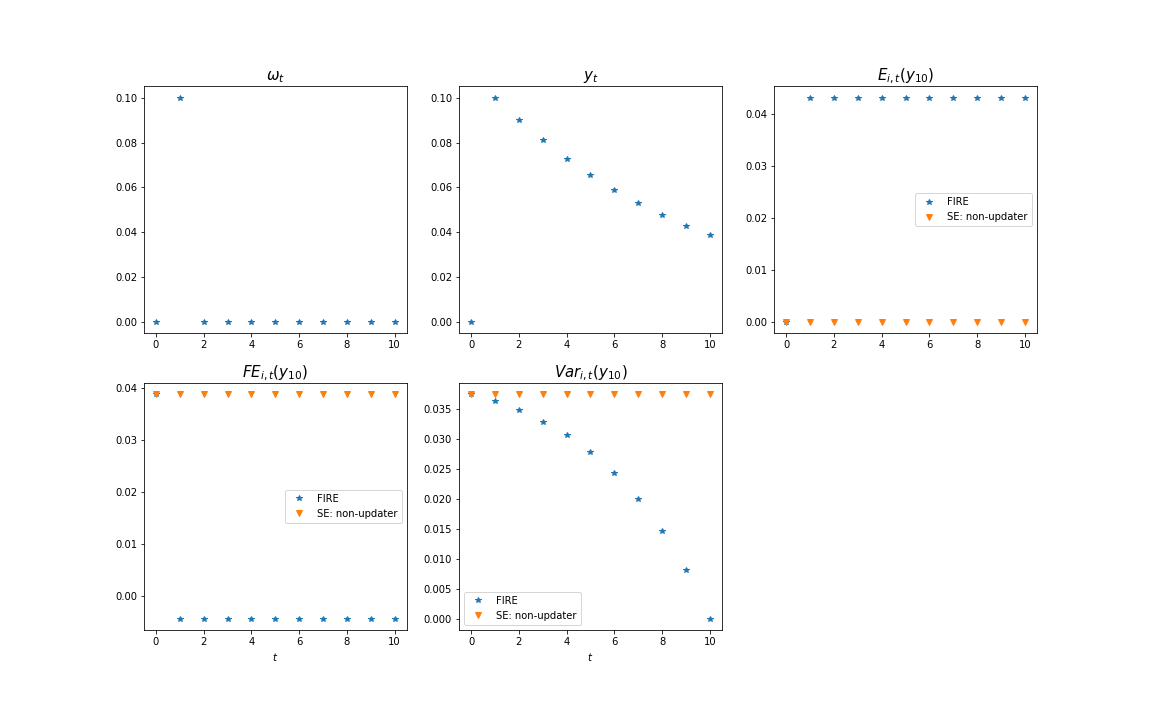
\includegraphics[scale=0.25]{figures/ir_indse} 
\end{figure}
\end{frame}


\begin{frame}{Impulse responses to shocks: population moments}

$$\textrm{True Process} \quad  \rho=0.9, \quad \sigma_\omega=0.1, \quad \omega_1 = 0.1$$
$$\textrm{SE} \quad \quad  \lambda = 0.4 $$ 

\begin{figure}
	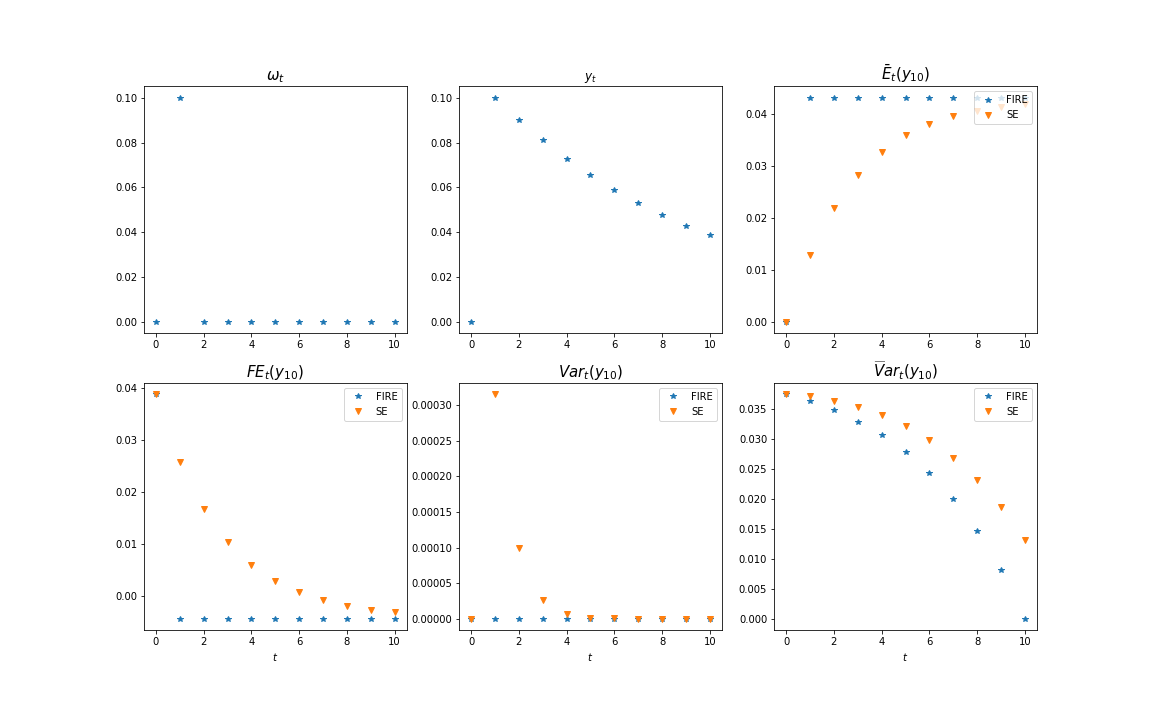
\includegraphics[scale=0.25]{figures/ir_popse} 
\end{figure}

\end{frame}

\subsection{Other theories}

\begin{frame}{Noisy Information: assumptions}
\begin{itemize}
	\item Individual only observes noisy signals 
	\begin{eqnarray*}
		\begin{aligned}
			& s_{i,t}=[s^{pb}_t, s^{pr}_{i,t}]' \in I_{i,t} \\
			&\text{public signal:} \quad s^{pb}_t = y_t + \epsilon_t, \quad \epsilon_t \sim N(0,\sigma^2_\epsilon)\\ 
			& \text{private signal:} \quad s^{pr}_{i,t} = y_t + \xi_{i,t} \quad \xi_{i,t} \sim N(0,\sigma^2_\xi)
		\end{aligned}
	\end{eqnarray*} 
   
	\item Kalman filtering (simply normal updating if $\rho$=0)
\end{itemize}
\end{frame}



\begin{frame}{Impulse responses to shocks: individual moments}


$$\textrm{True Process} \quad   \rho=0.9, \quad \sigma_\omega= 0.1, \quad \omega_1 = 0.1$$
$$ \textrm{SE:} \quad  \lambda = 0.5; \quad \textrm{NI:} \quad \sigma_\xi = 0.1, \quad \sigma_\epsilon = 0.1$$

\begin{figure}
	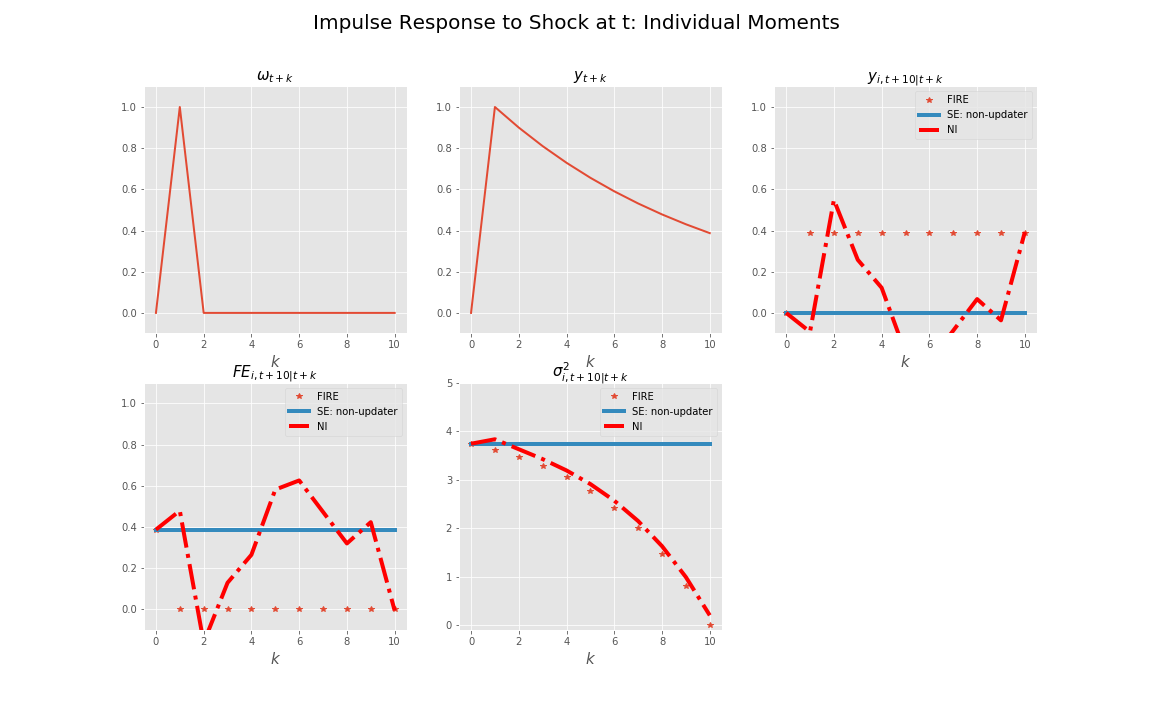
\includegraphics[height=6.3cm,width=10cm]{figures/ir_indseni} 
\end{figure}

\end{frame}

\begin{frame}{Impulse responses to shocks: population moments}


$$\textrm{True Process} \quad   \rho=0.9, \quad \sigma_\omega= 0.1, \quad \omega_1 = 0.1$$
$$ \textrm{SE:} \quad  \lambda = 0.5; \quad \textrm{NI:} \quad \sigma_\xi = 0.1, \quad \sigma_\epsilon = 0.1$$

\begin{figure}
	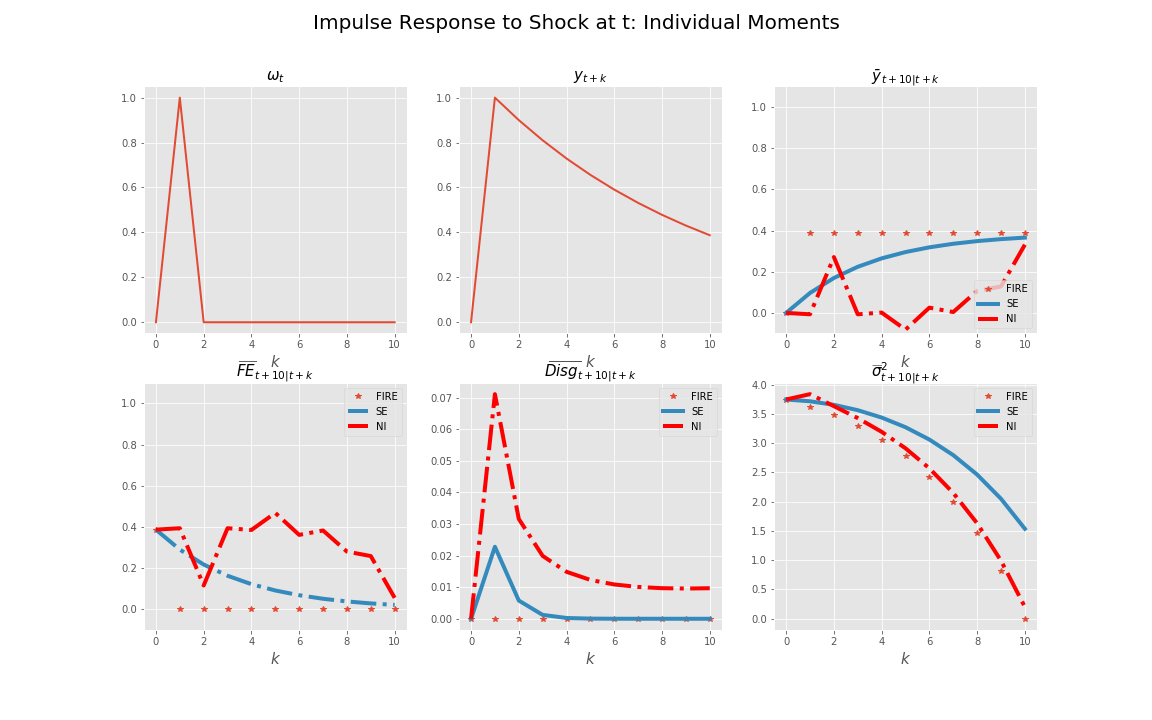
\includegraphics[height=6.3cm,width=10cm]{figures/ir_popseni} 
\end{figure}

\end{frame}

%\begin{frame}{Noisy Information: predictions}
%\begin{itemize}
%	\item \textbf{Similar to Sticky Expectation}
%	\begin{enumerate}
%\item \textbf{Macro rigidity}: population forecasts partially respond to shocks
% \item \textbf{Non-response of variance}: both individual and population variance \textcolor{blue}{does not respond to} shocks.   
% \end{enumerate}
%\item \textbf{Different from Sticky Expectation}

%	\begin{enumerate}
%	\item \textbf{Micro rigidity}: both individual and population forecast \textcolor{blue}{partially} respond to shocks 
%	\item \textbf{Horizon-sensitive rigidity}: rigidity decreases with horizon
%	\item \textbf{Increasing disagreements:} population disagreements \textcolor{blue}{increase} over time as approaching $t+h$
%	\item \textbf{Shock-specific responses:} different impacts of fundamental shocks, or simply news shocks 
%\end{enumerate}
%\end{itemize}

%\end{frame}


\begin{frame}{A detailed look into noisy information}


\begin{figure}
	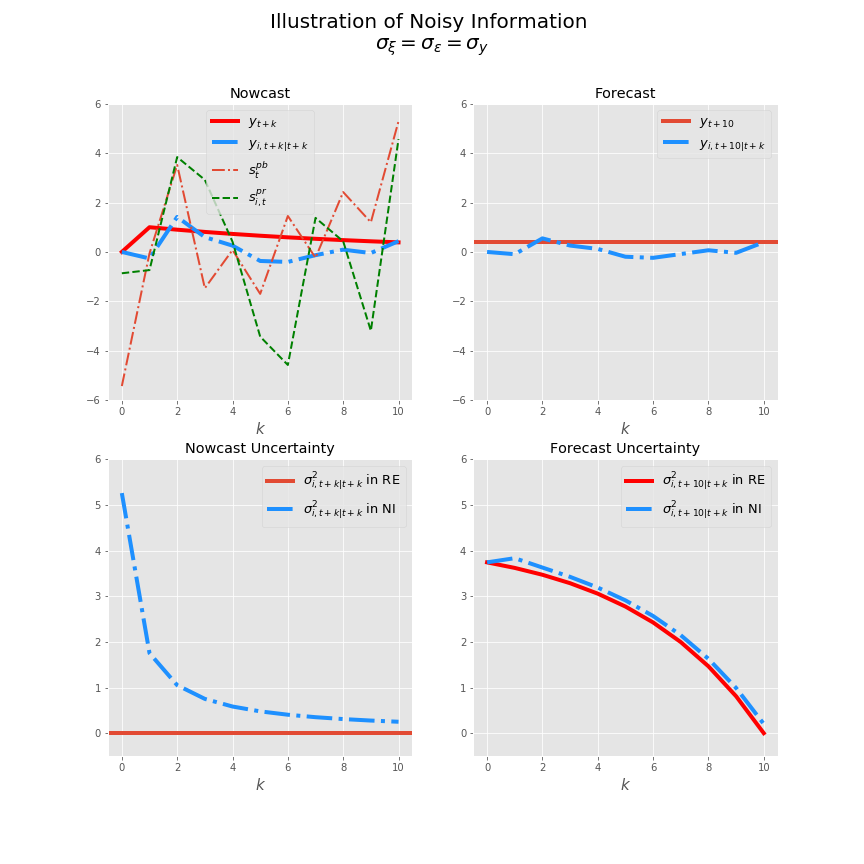
\includegraphics[height=8cm,width=8cm]{figures/ni_illustration} 
\end{figure}

\end{frame}


\begin{frame}{Implied rigidity of different models}


\begin{figure}
	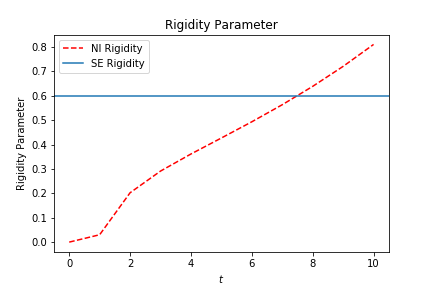
\includegraphics[height=5cm,width=8cm]{figures/rigidity} 
\end{figure}

\end{frame}



\begin{frame}{Other theories on to-do-list}
\begin{itemize}
	\item \textbf{Rational Inattention:} attentiveness endogenously respond to variances
	\item \textbf{Learning}: the structural parameter $\rho$ is not known, thus the agent learns about it as if an econometrician does
\end{itemize}
\end{frame}

\begin{frame}{Identification strategies 1: testing rigidity models}

\begin{itemize}
	\item\cite{coibion2012can}
	\begin{itemize}
		\item \textcolor{blue}{FEs} respond to shocks and serially correlated. 
	\end{itemize}
	\item \textbf{Additional in this paper}
	\begin{itemize}
		\item \textcolor{blue}{Uncertainty} does not depend on shocks; and serially correlated. 
	\end{itemize}
\end{itemize}

\end{frame}

\begin{frame}{Identification strategies 2: differentiating theories}
\begin{itemize}
	\item\cite{coibion2012can}
	\begin{itemize}
		\item \textcolor{blue}{FEs} do not depend on past realizations according to baseline SE and NI; but do so according to heterogeneous priors or precision models. 
		\item Implied rigidity does not differ across shocks according to SE but differs according to NI. 
		\item \textcolor{blue}{Disagreements} rise after shocks according to baseline SE, strategic interactions and heterogeneous priors but invariant according to baseline NI.
	\end{itemize}
	\item \textbf{Additional in this paper}
	\begin{itemize}
		\item \textcolor{blue}{Uncertainty} do not depend on shocks per se according to baseline SE and NI, instead on degree of information rigidity.
	\end{itemize}
\end{itemize}

\end{frame}

\section{Data and Methodology}


\begin{frame}{Data}
\begin{table}[]
\resizebox{\textwidth}{!}{	\begin{tabular}{lll}
		
		\hline 
		& SCE & SPF        \\
		\hline 
		Time period                                    & 2013-present                            & 2007-present             \\
		Frequency                                      & Monthly                                 & Quarterly                \\
		Sample Size                                    & 1,300                                   & 30-50                    \\
		Aggregate Var in Density                       & \textcolor{blue}{1-yr and 3-yr inflation}          & \textcolor{blue}{1-yr and 3-yr CPI and PCE}         \\
		Pannel Structure                               & stay up to 12 months                    & average stay for 5 years \\
		Demographic Info                        & Education, Income, Age        & Industry    \\
		\hline 
	\end{tabular}}
\end{table}

\end{frame}



\section{Stylized Facts}

\begin{frame}{Population moments: average}
\begin{figure}
	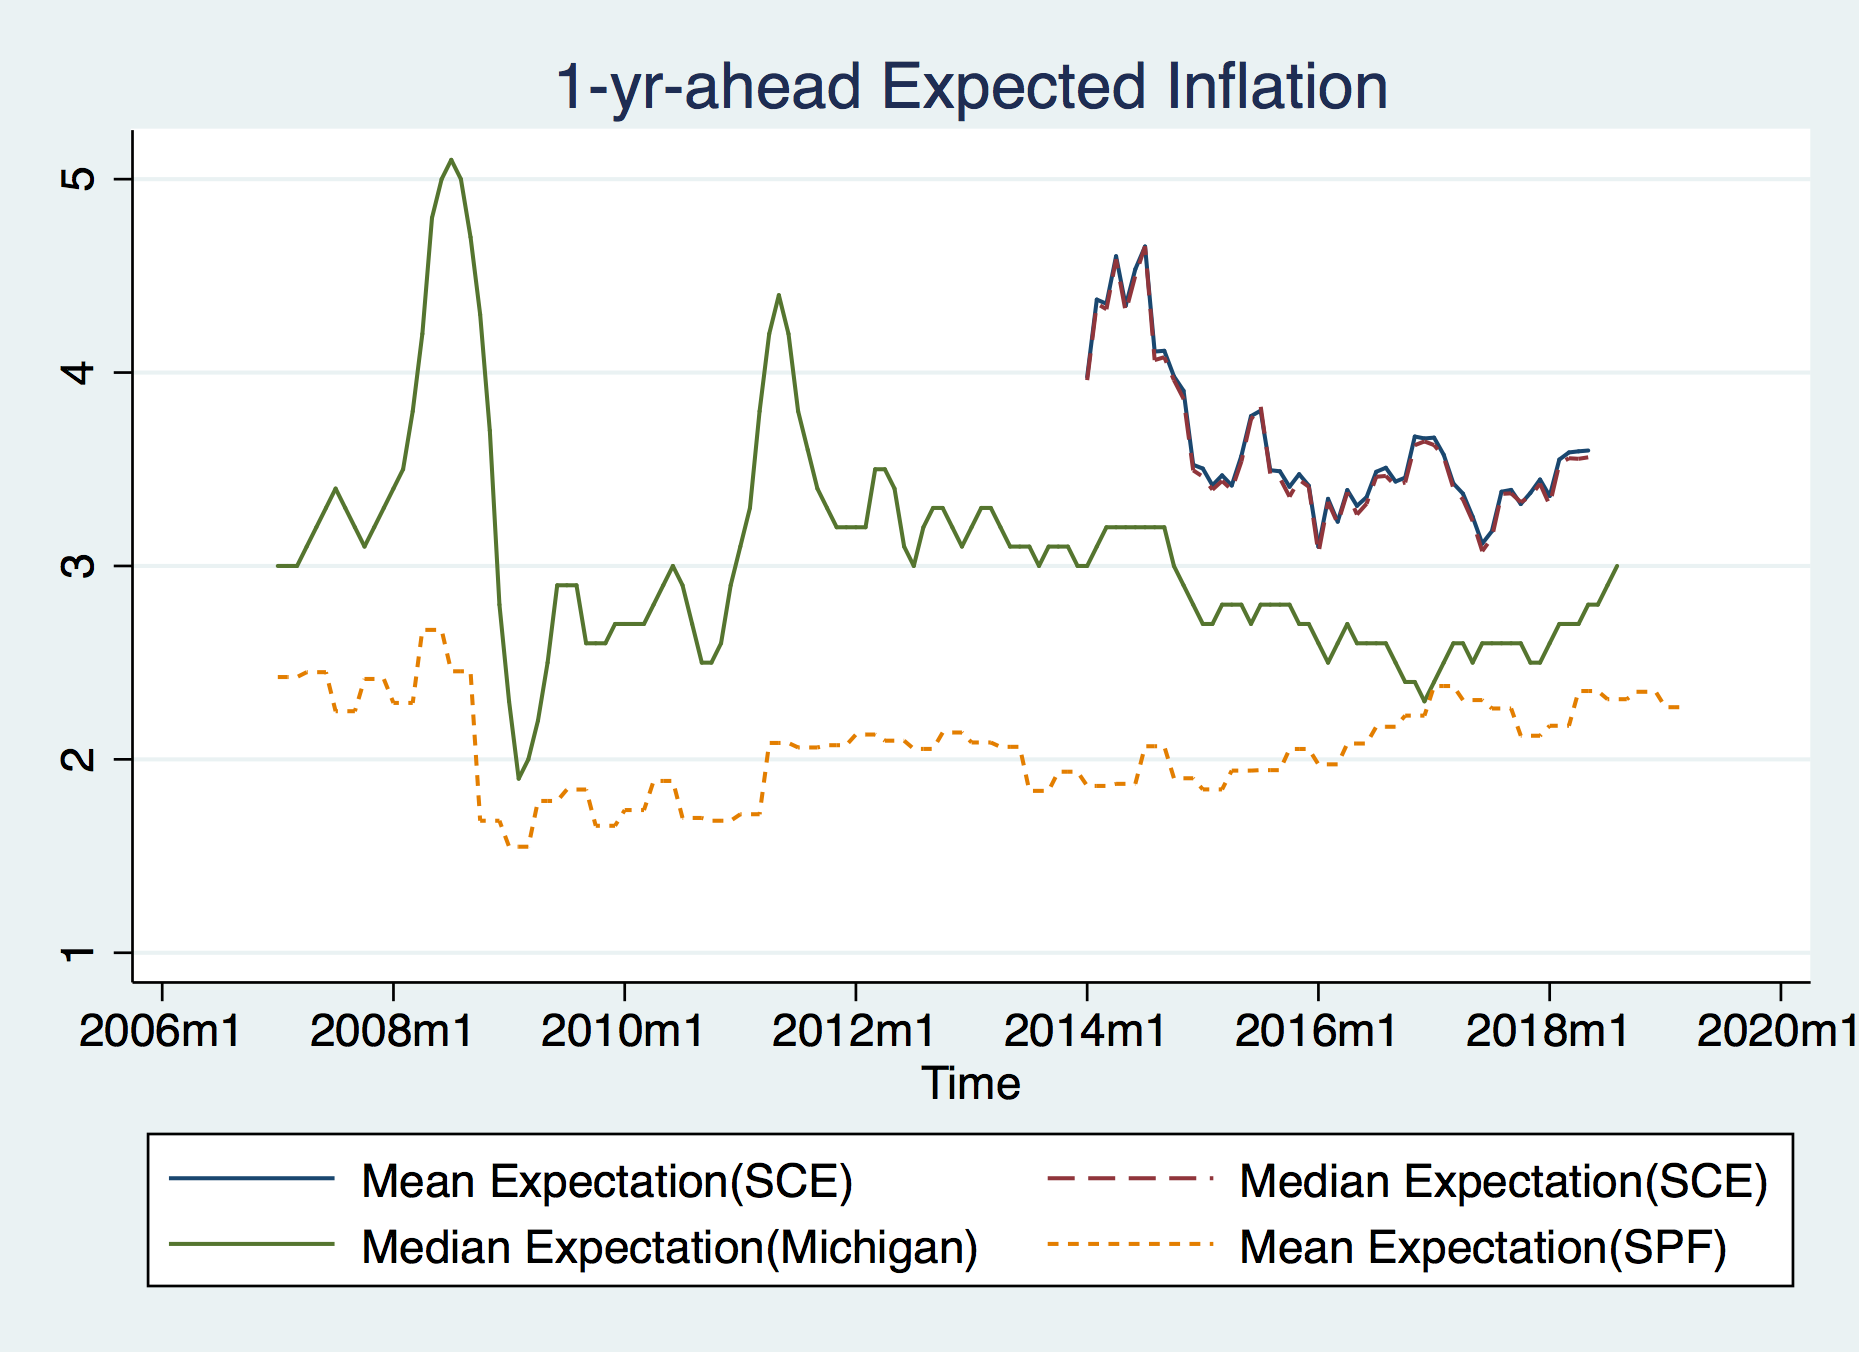
\includegraphics[scale=0.3]{figures/mean_med.png} 
\end{figure}
\end{frame}


\begin{frame}{Population moments: average forecast errors}
\begin{figure}
	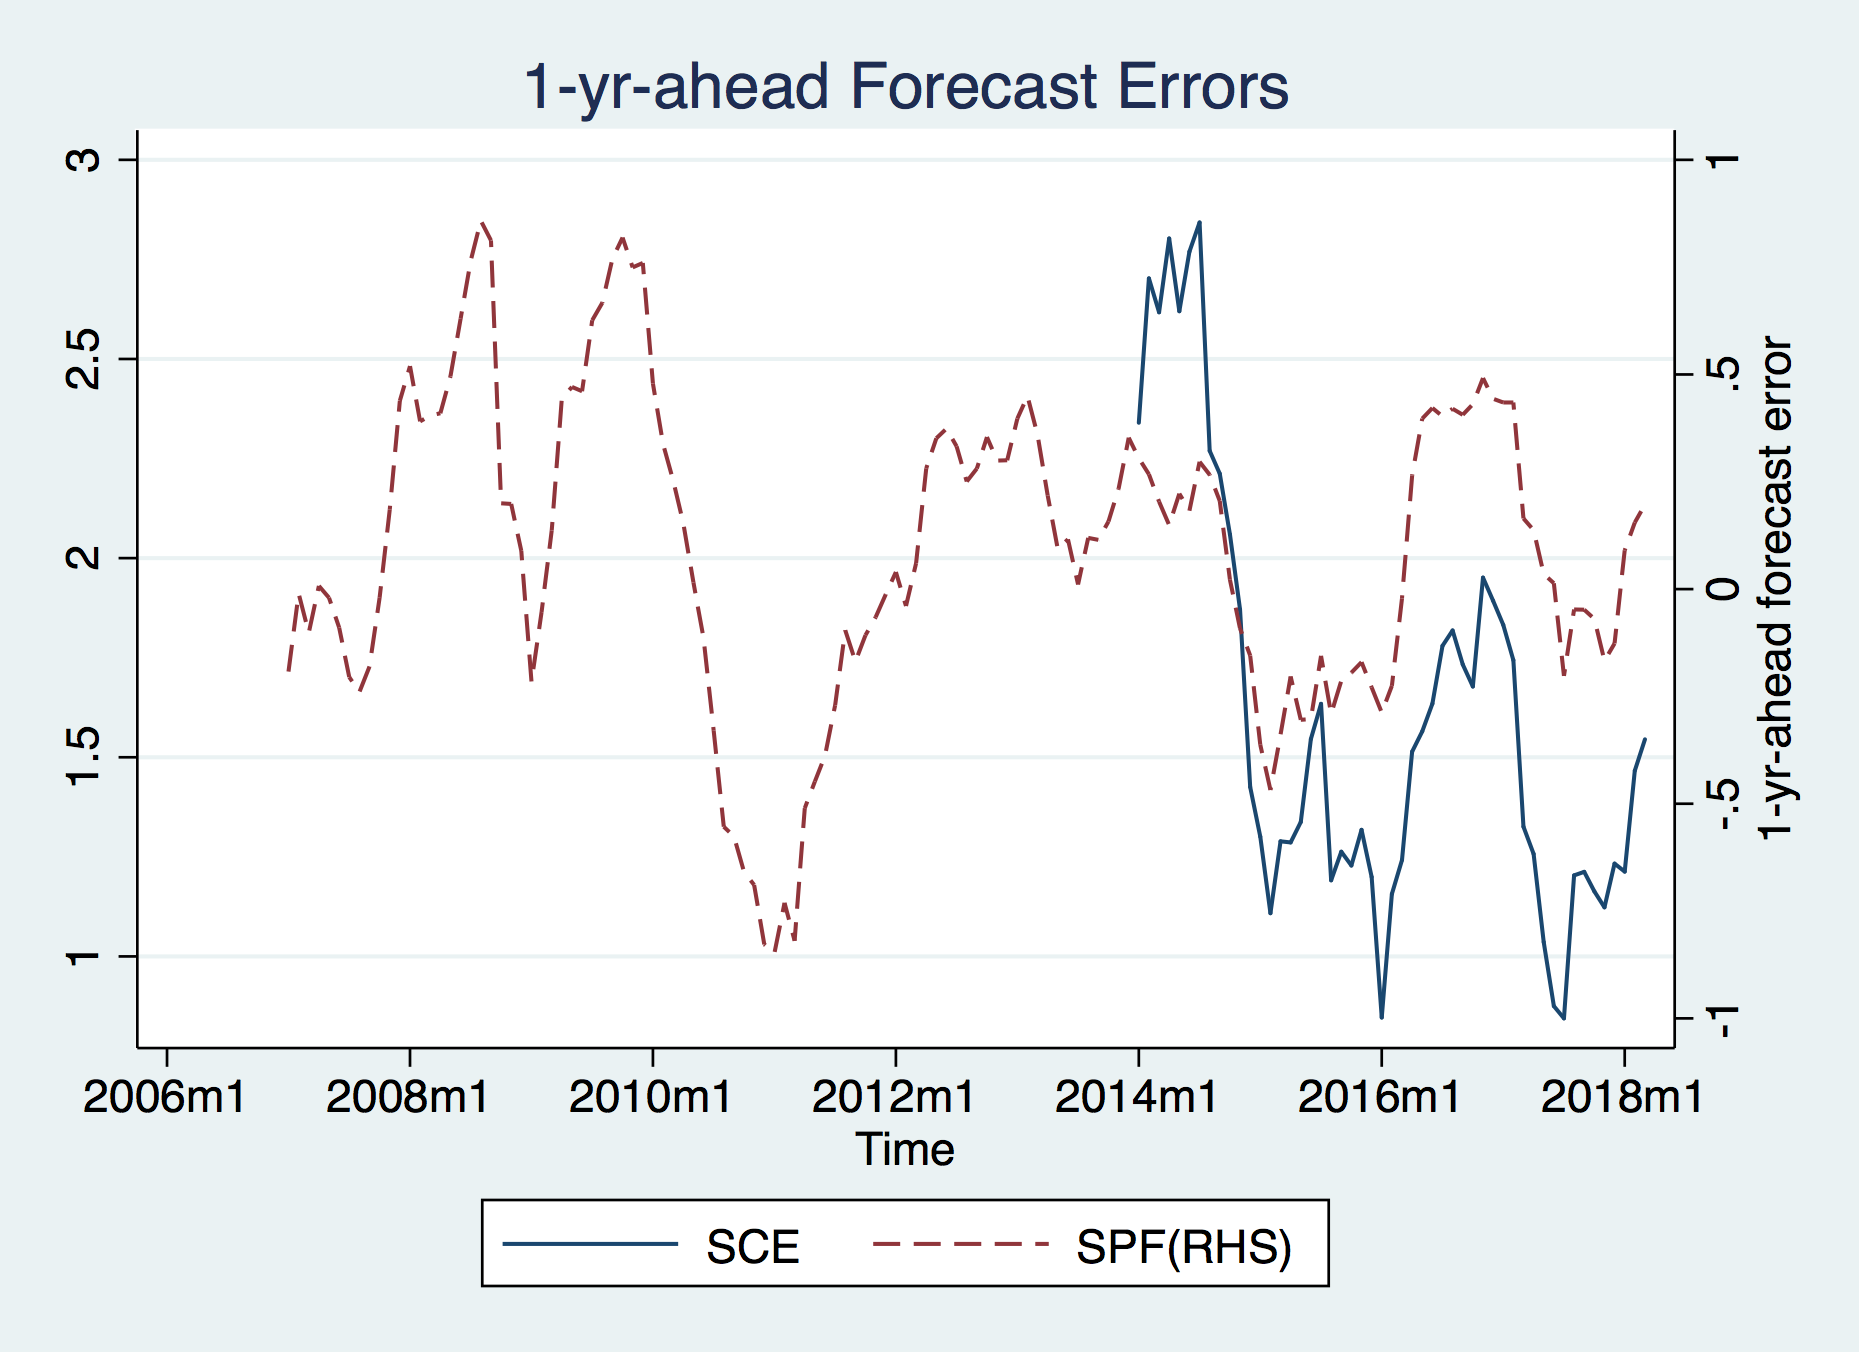
\includegraphics[scale=0.3]{figures/fe_fe.png} 
\end{figure}
\end{frame}

\begin{frame}{Population moments: average uncertainty}
\begin{figure}
	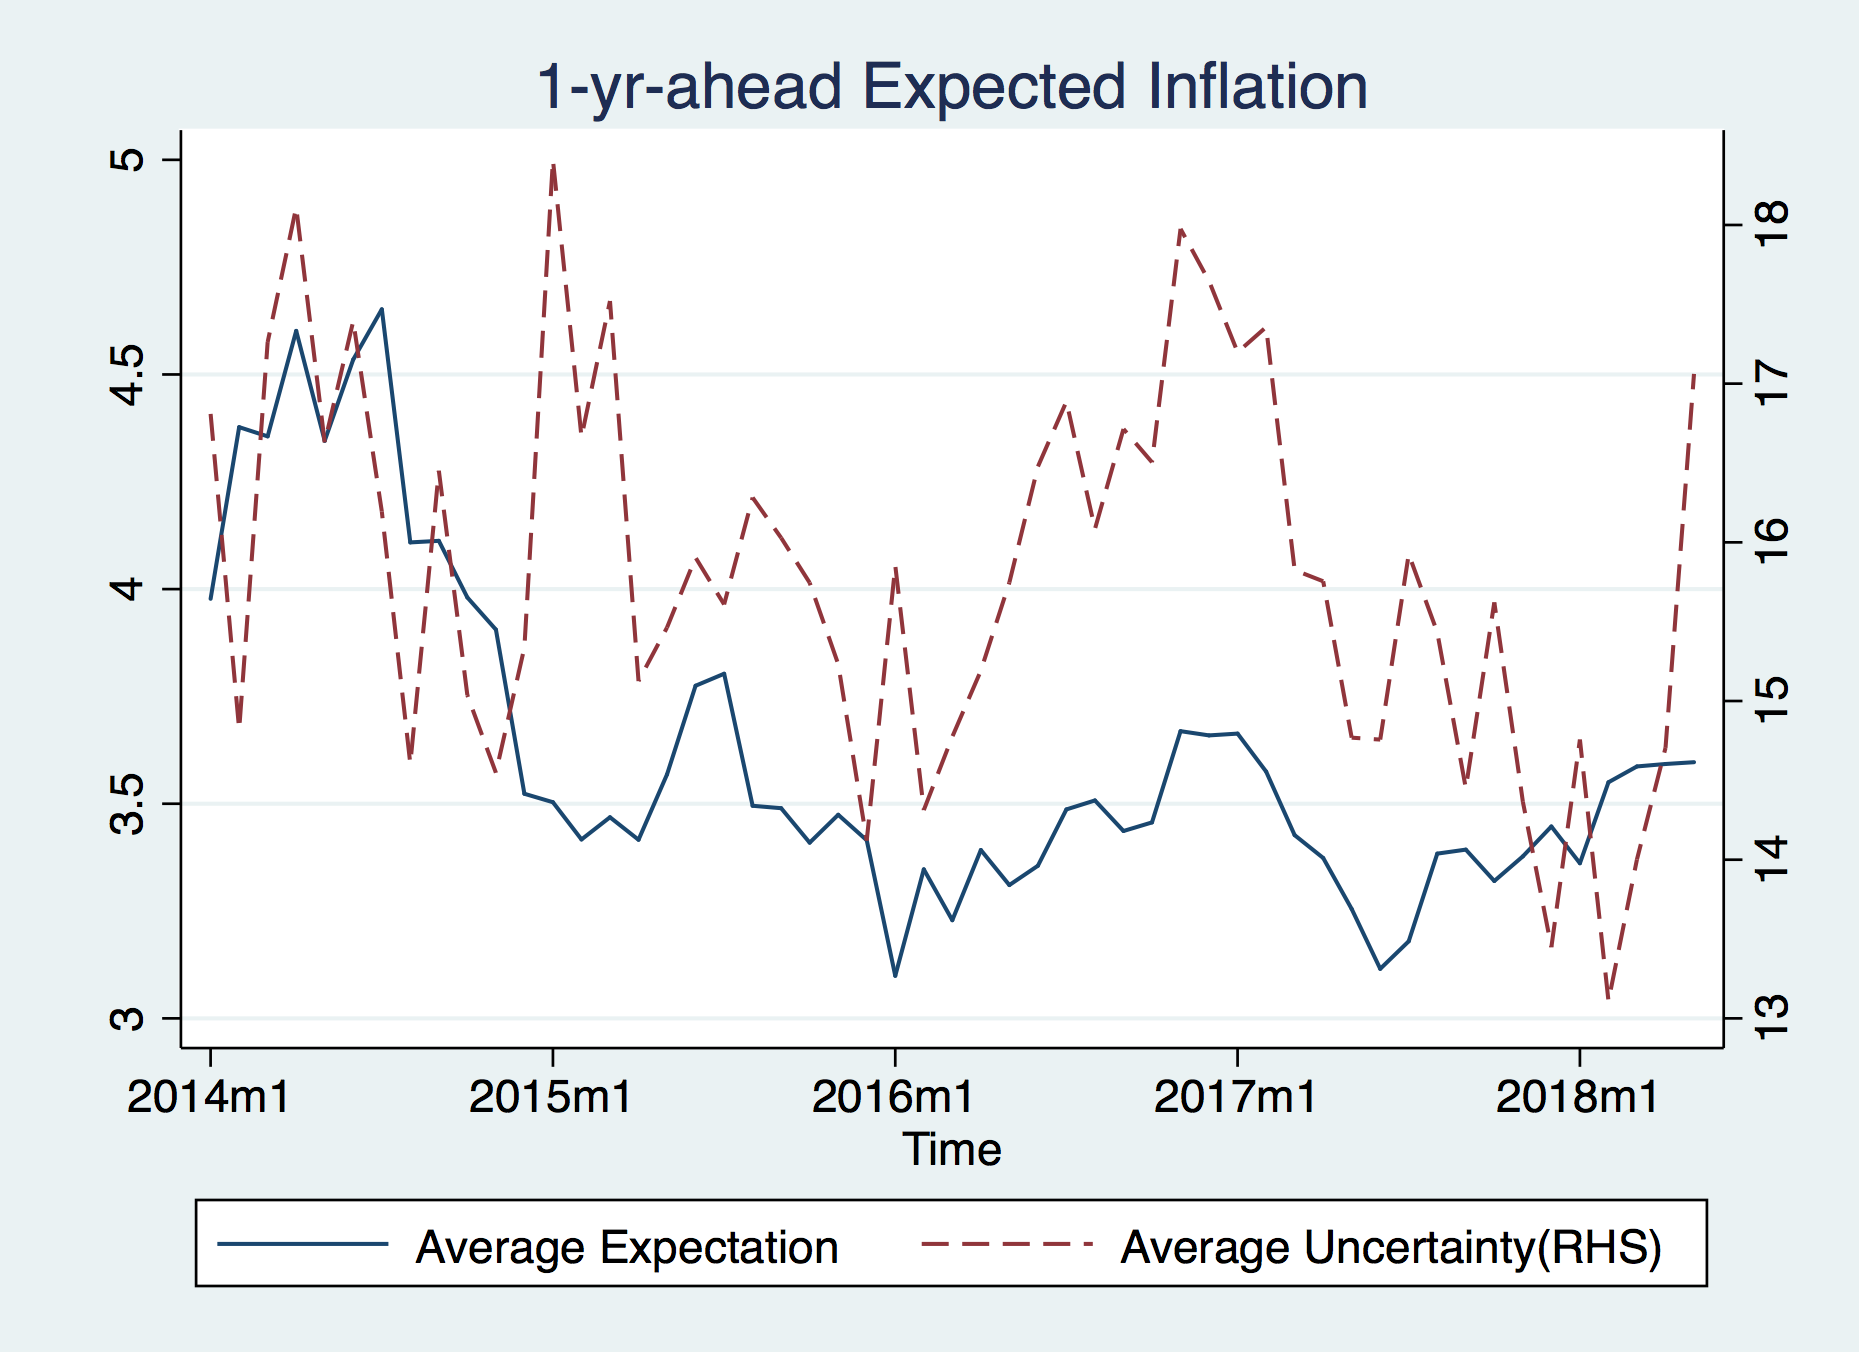
\includegraphics[scale=0.3]{figures/mean_var.png} 
\end{figure}
\end{frame}

\begin{frame}{Population moments: average uncertainty}
\begin{figure}
	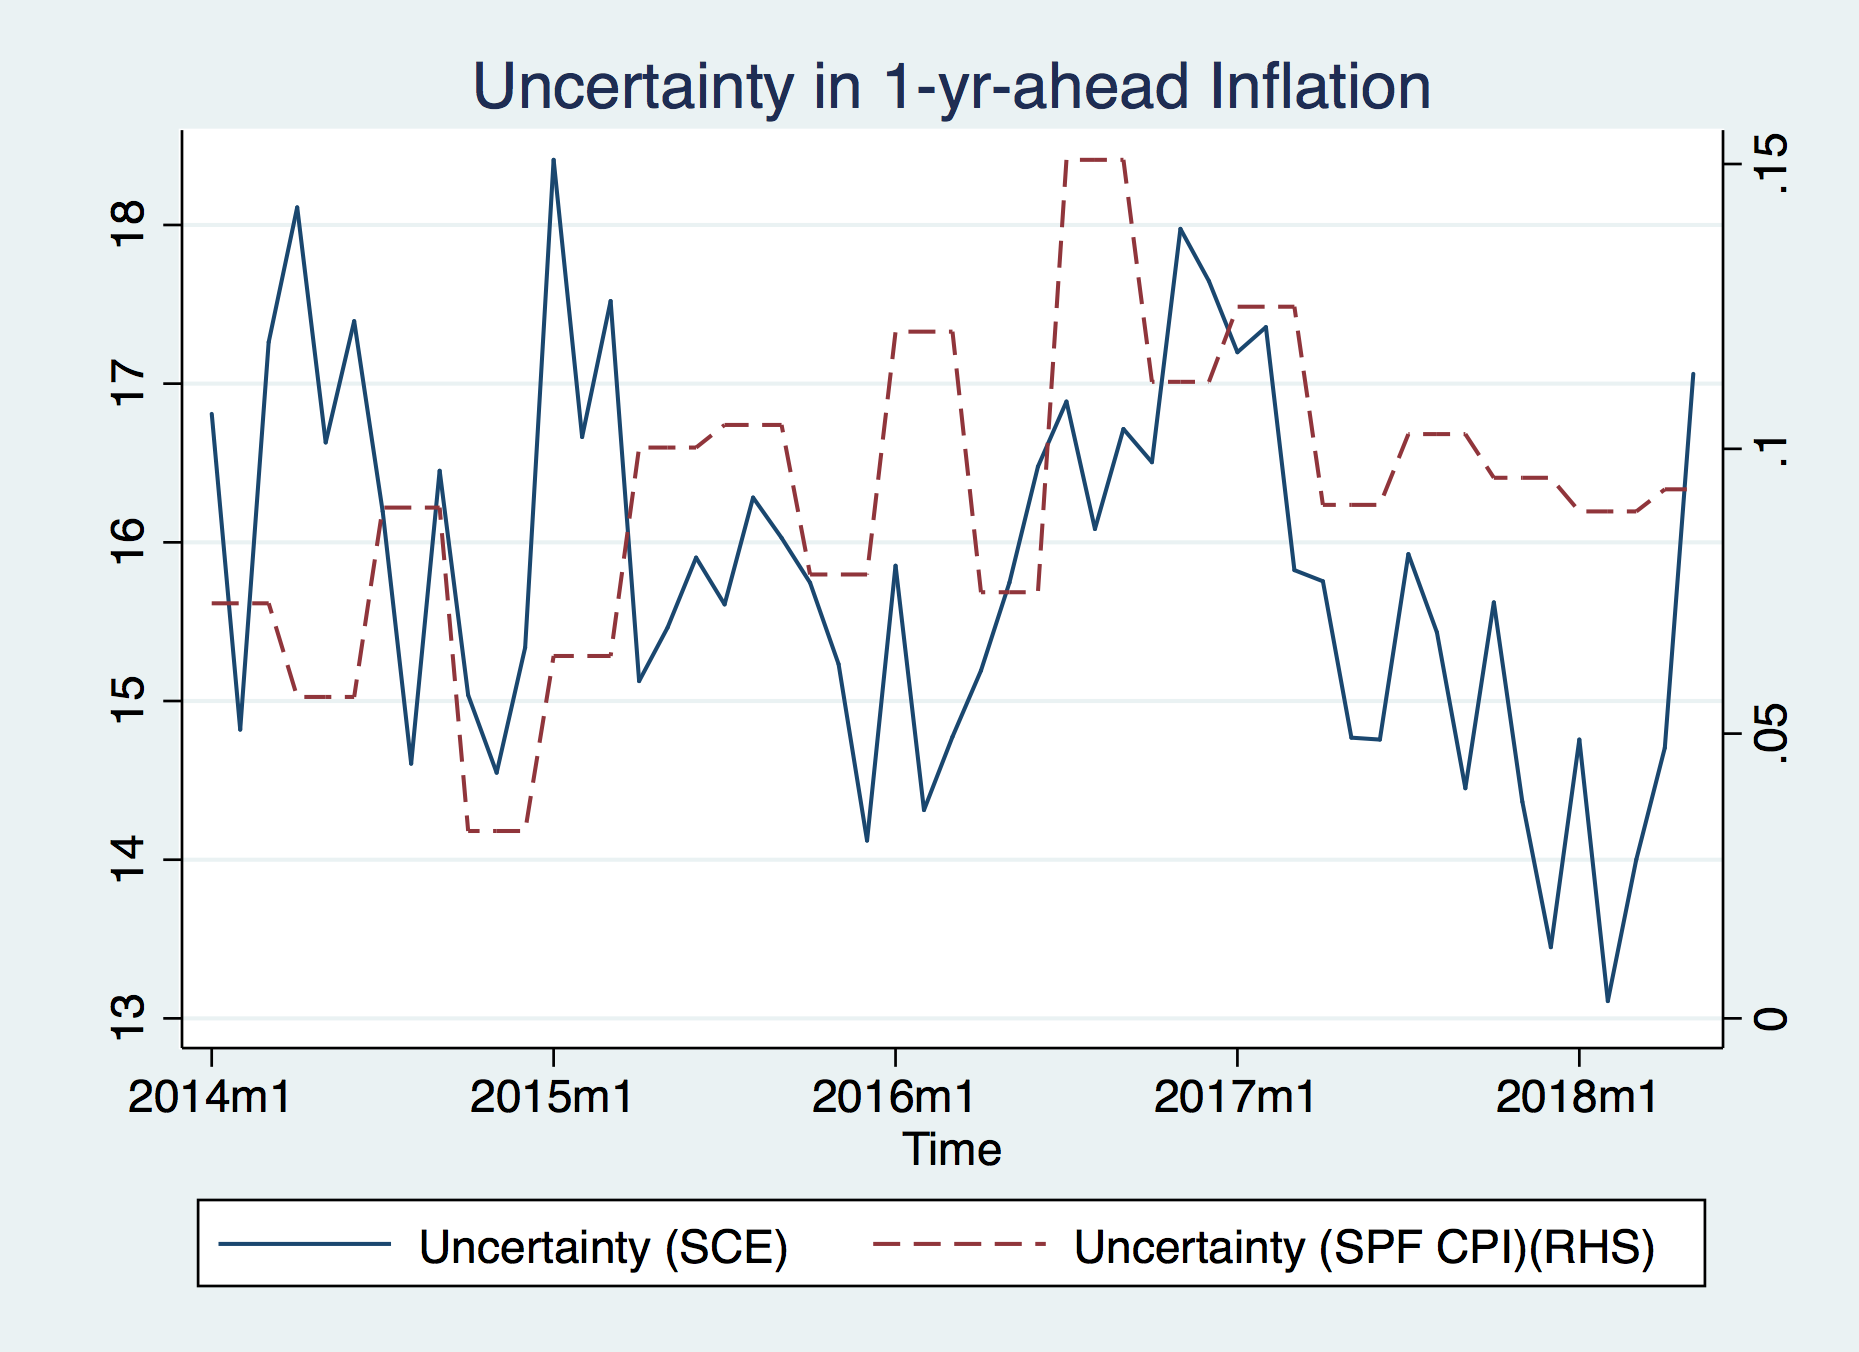
\includegraphics[scale=0.3]{figures/var_var.png} 
\end{figure}
\end{frame}


\begin{frame}{Population moments: disagreements}
\begin{figure}
	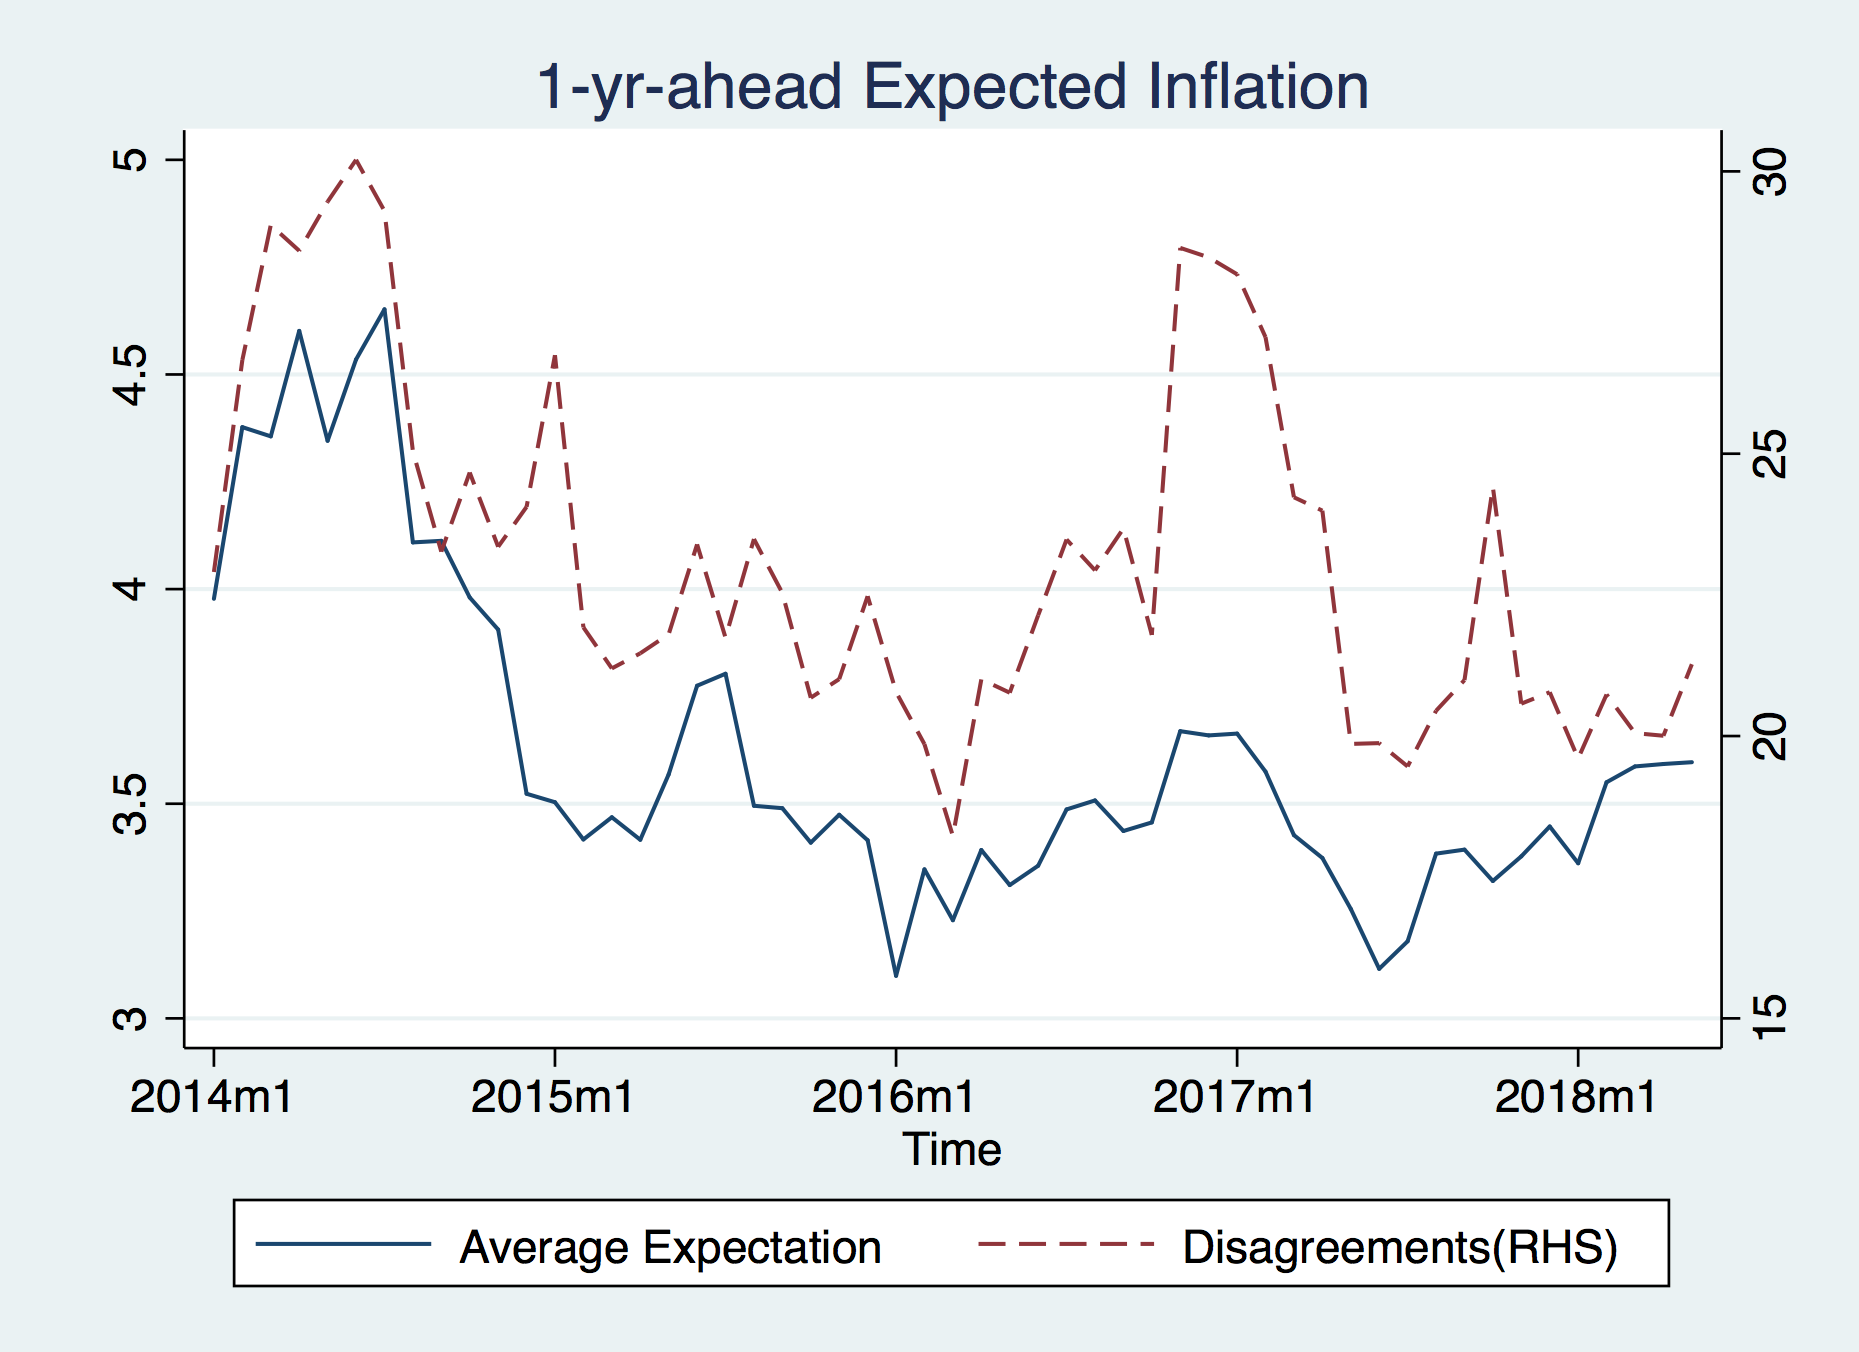
\includegraphics[scale=0.3]{figures/mean_disg.png} 
\end{figure}
\end{frame}


\begin{frame}{Population moments: disagreements}
\begin{figure}
	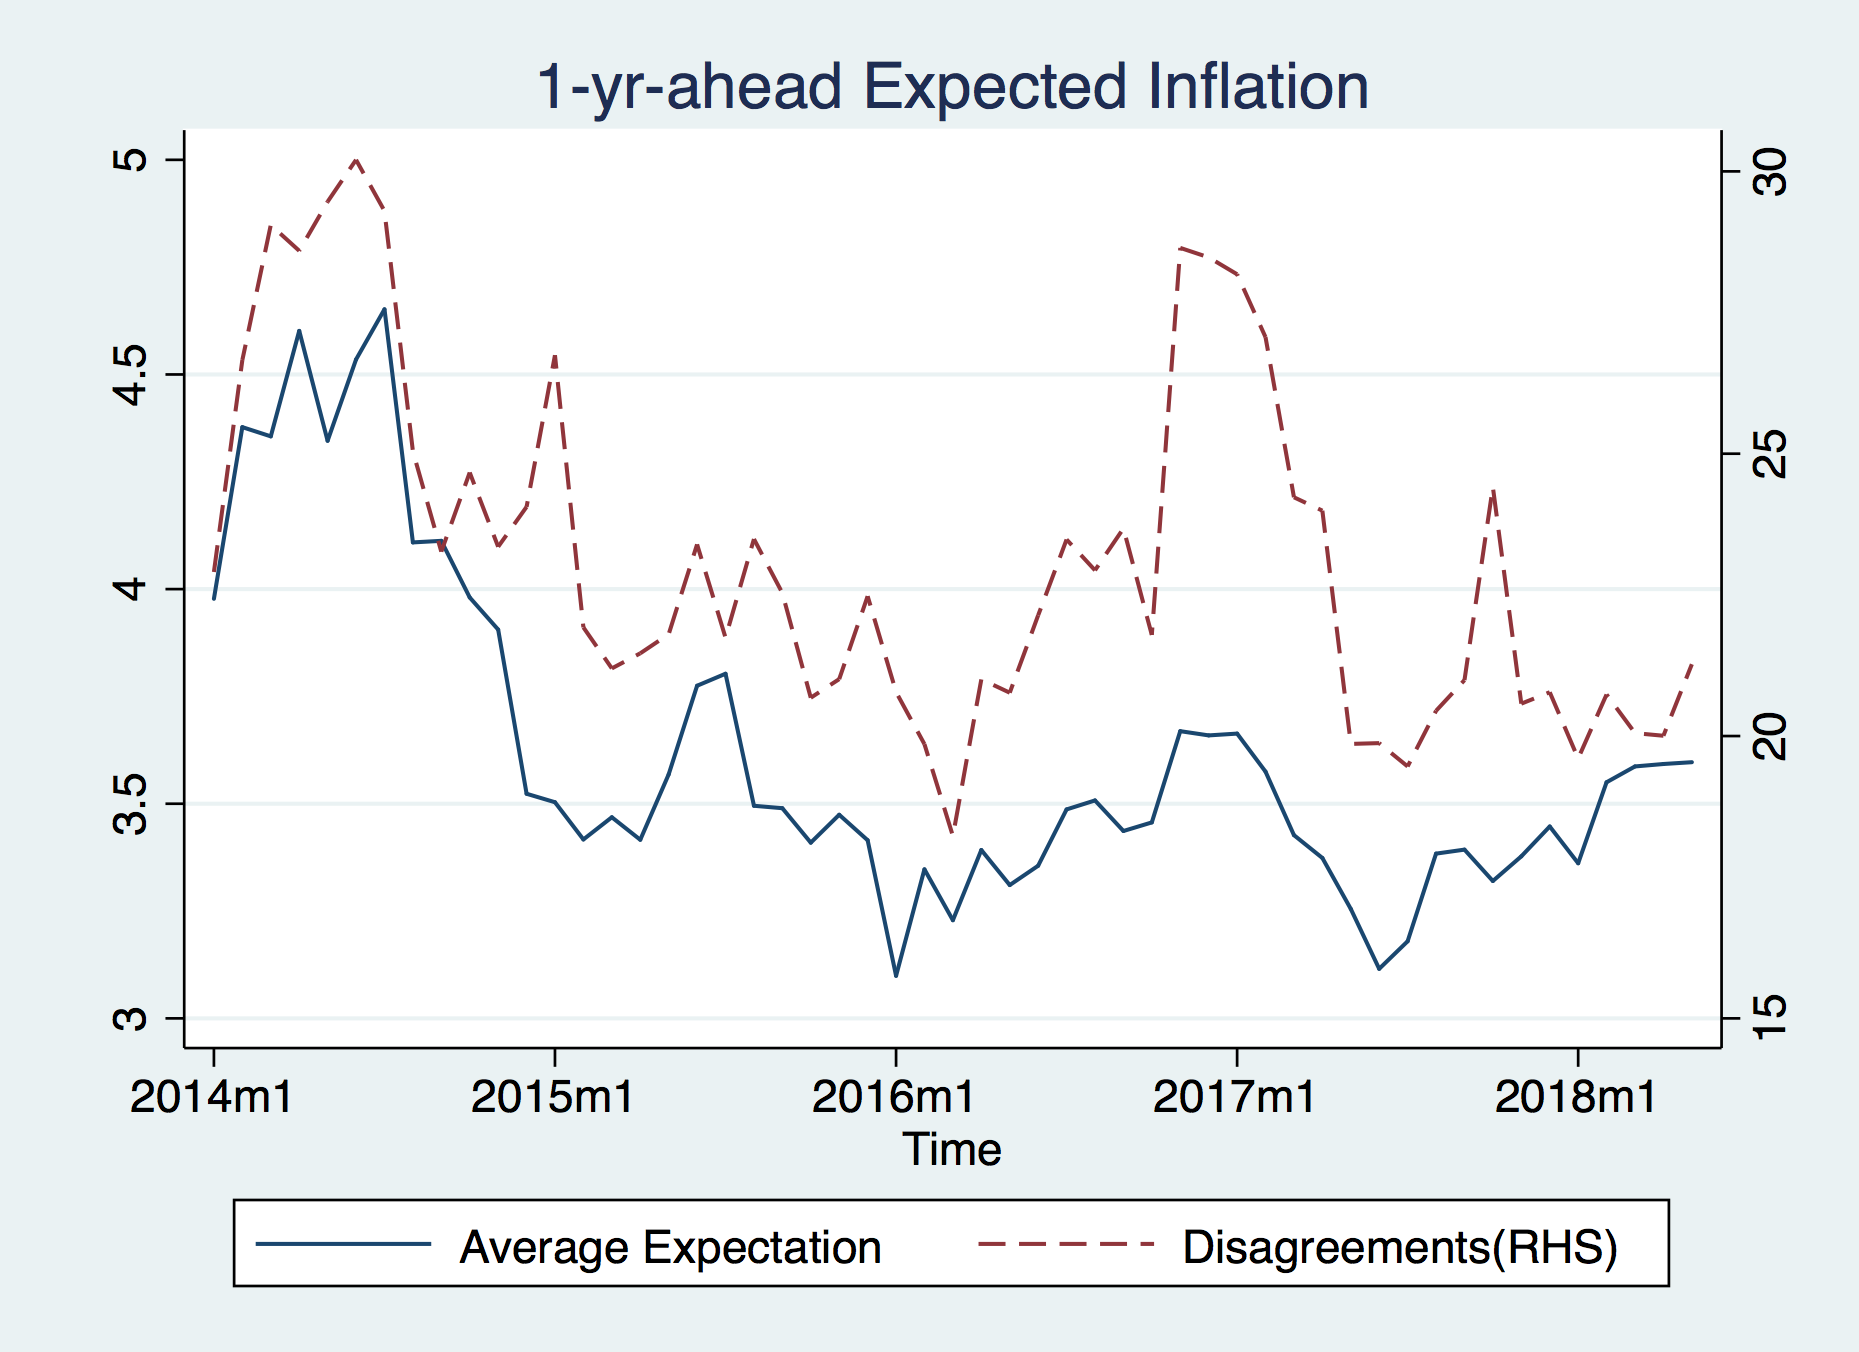
\includegraphics[scale=0.3]{figures/mean_disg.png} 
\end{figure}
\end{frame}


\begin{frame}{Population moments: disagreements}
\begin{figure}
	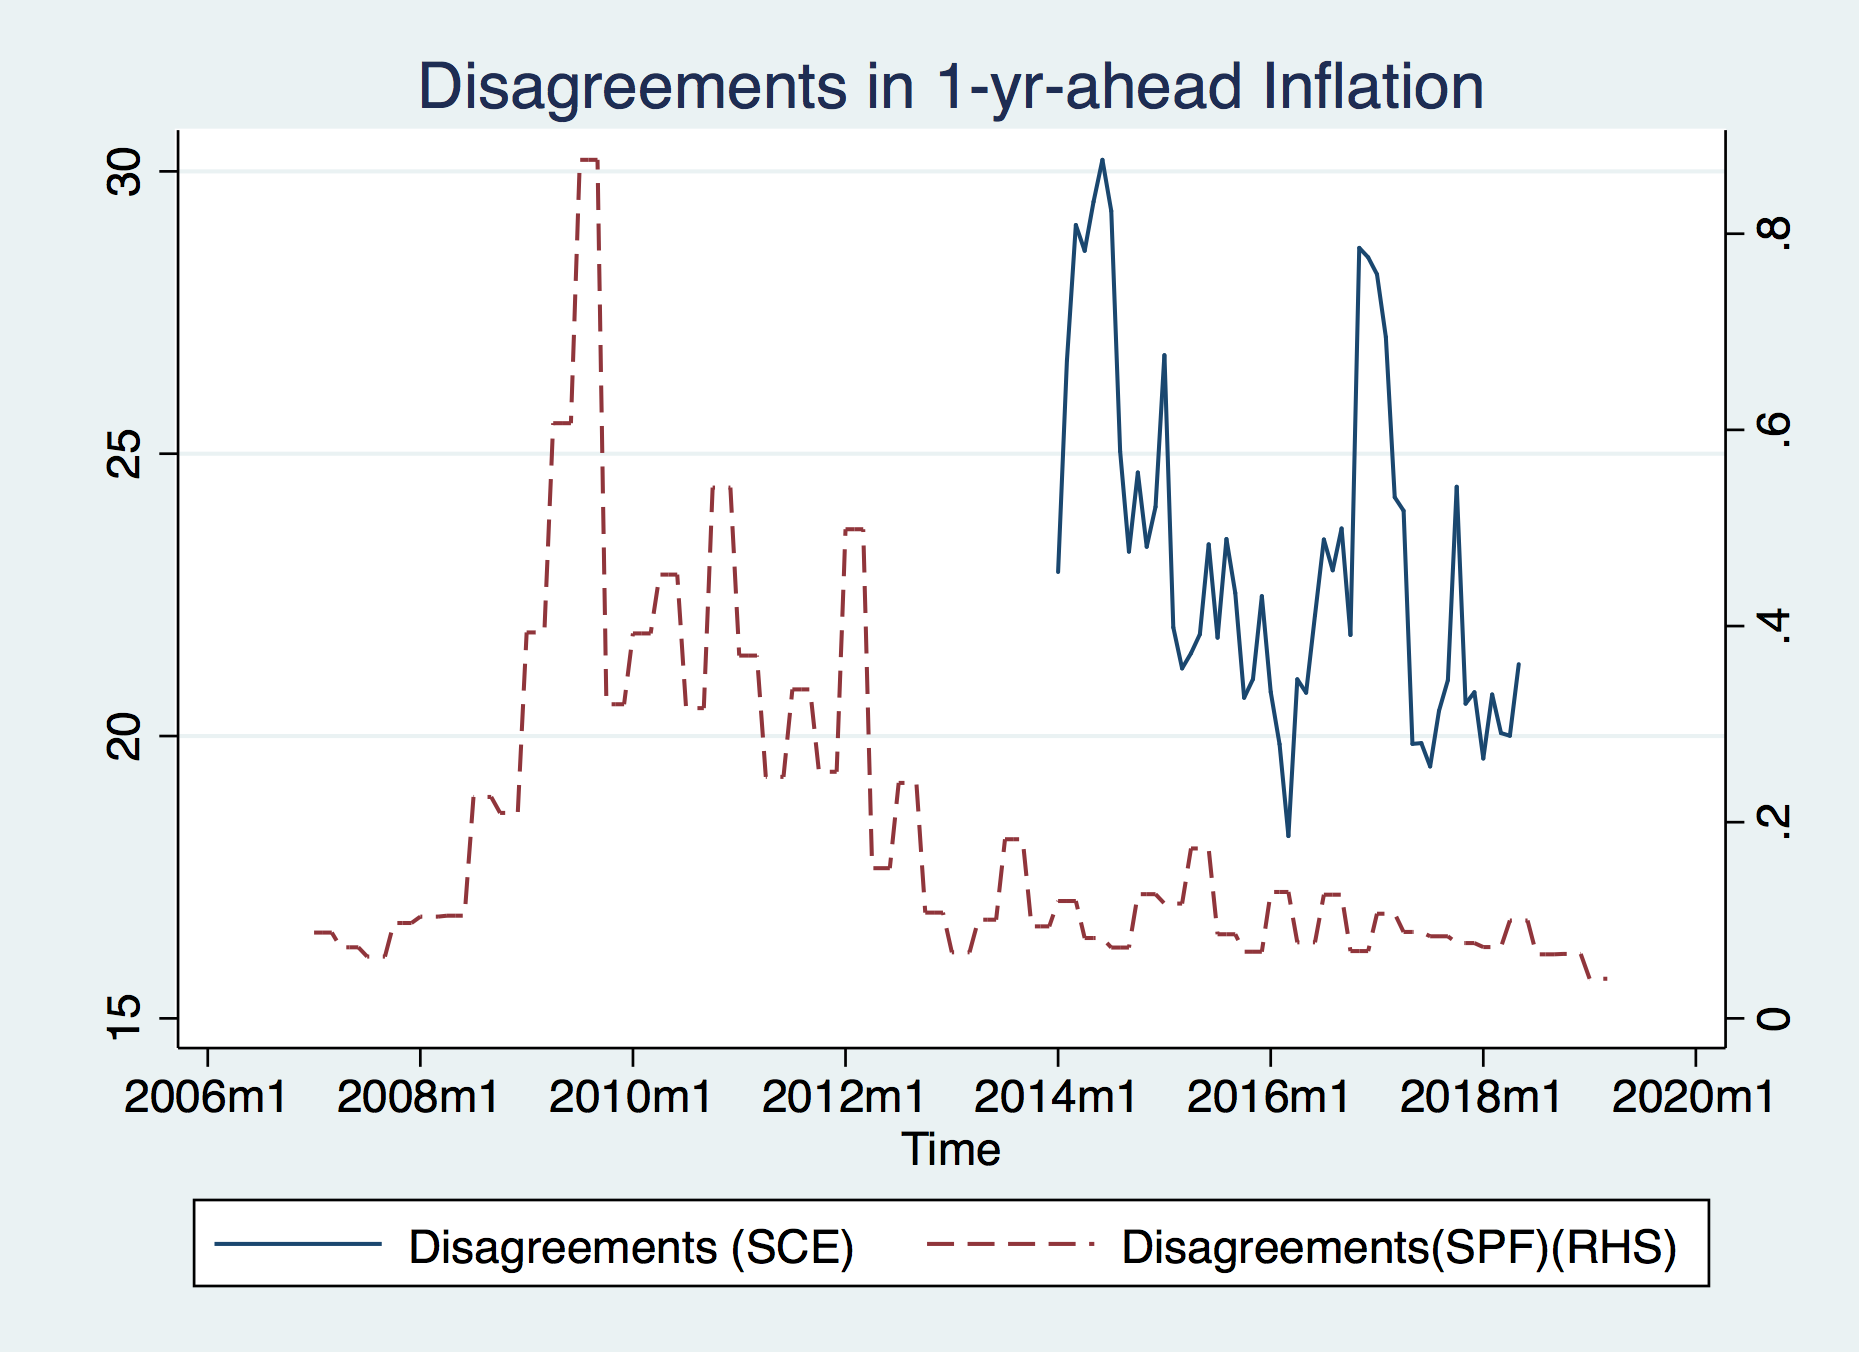
\includegraphics[scale=0.3]{figures/disg_disg.png} 
\end{figure}
\end{frame}


\begin{frame}{Population moments: uncertainty and disagreements}
\begin{figure}
	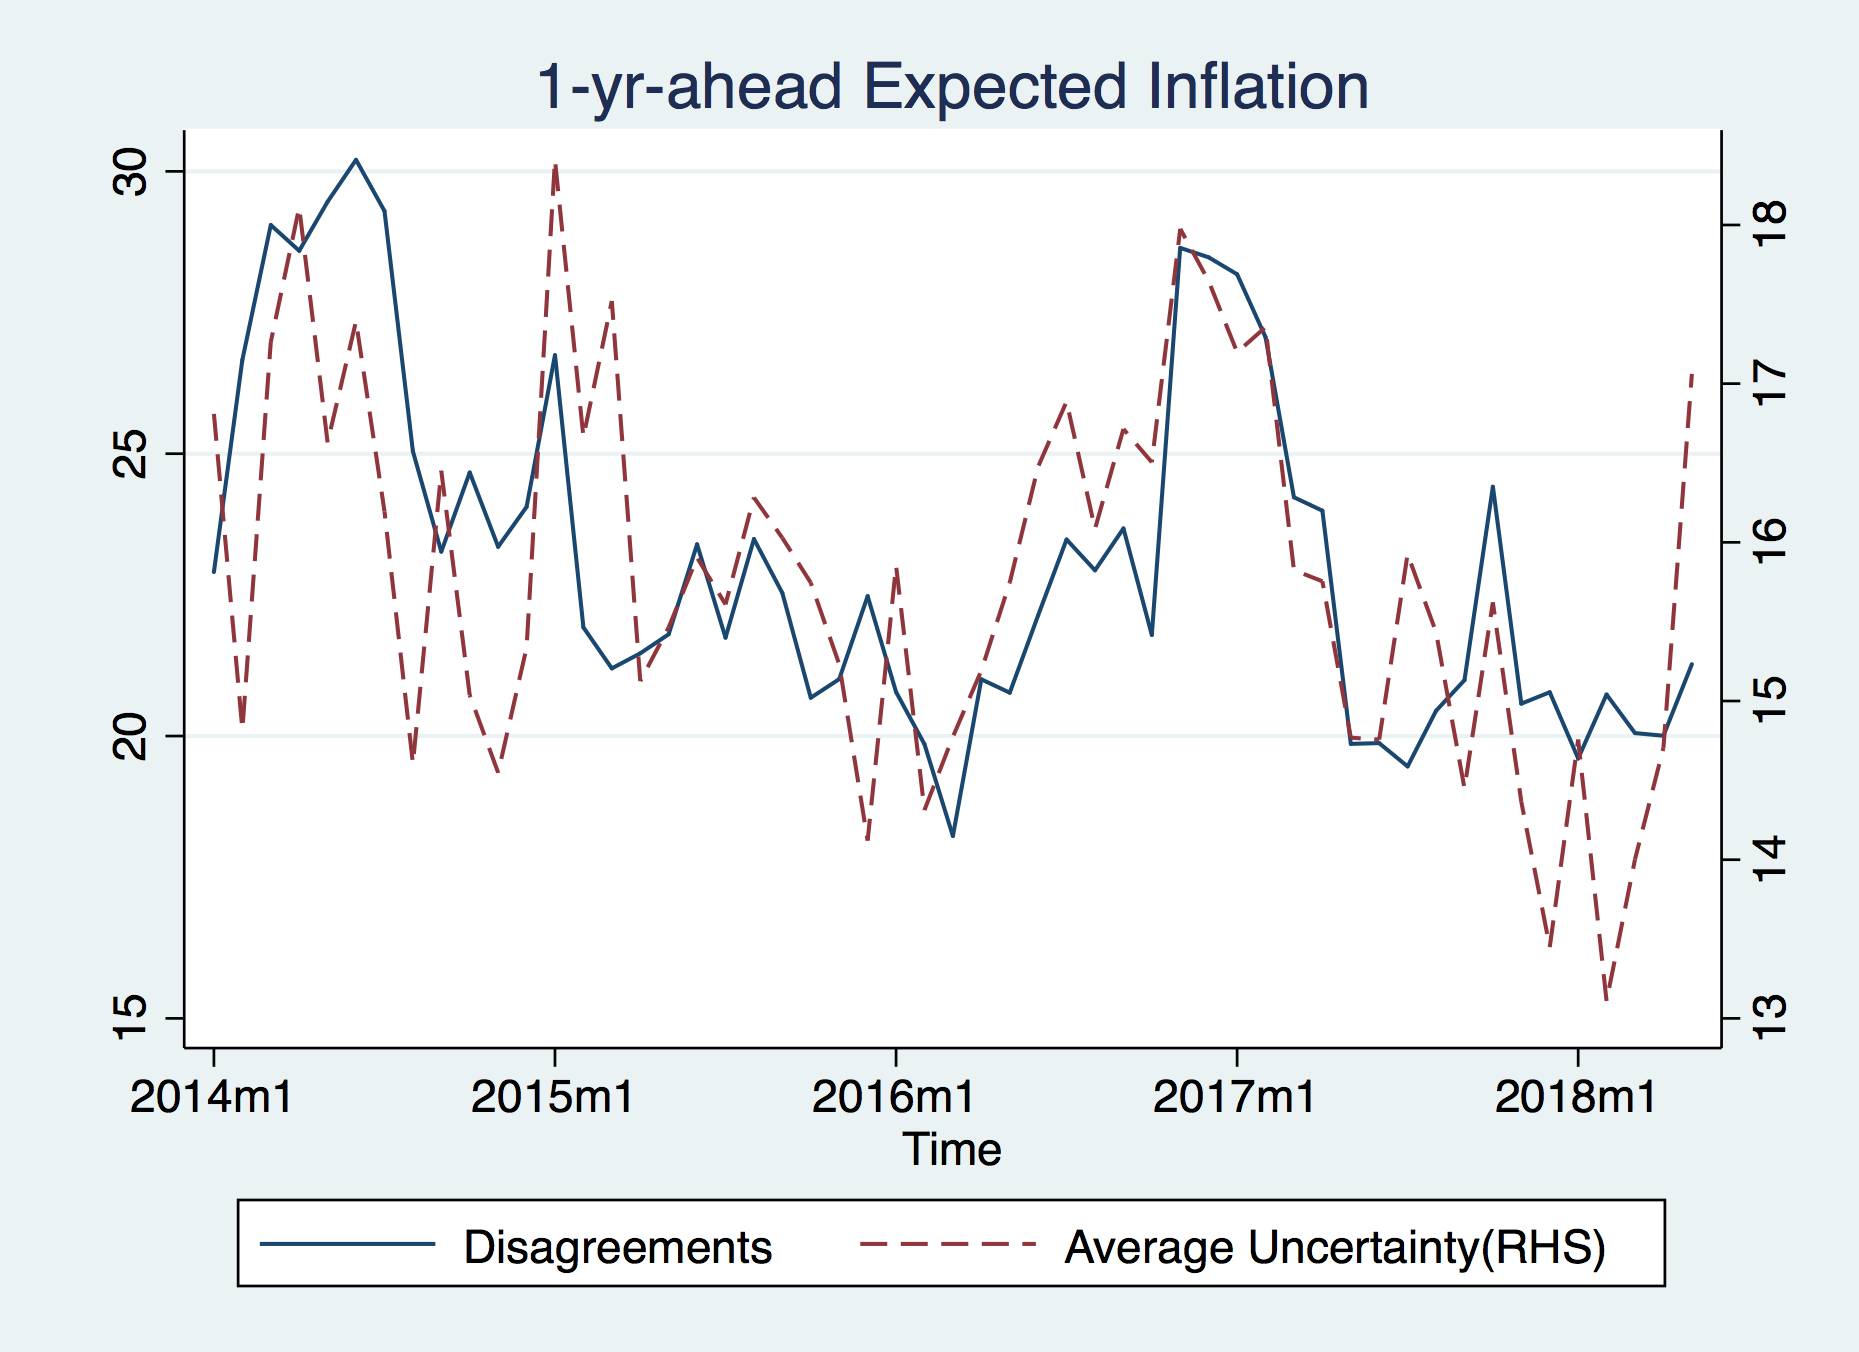
\includegraphics[scale=0.3]{figures/var_disg.png} 
\end{figure}
\end{frame}


\begin{frame}{Population moments: uncertainty and disagreements}
\begin{figure}
	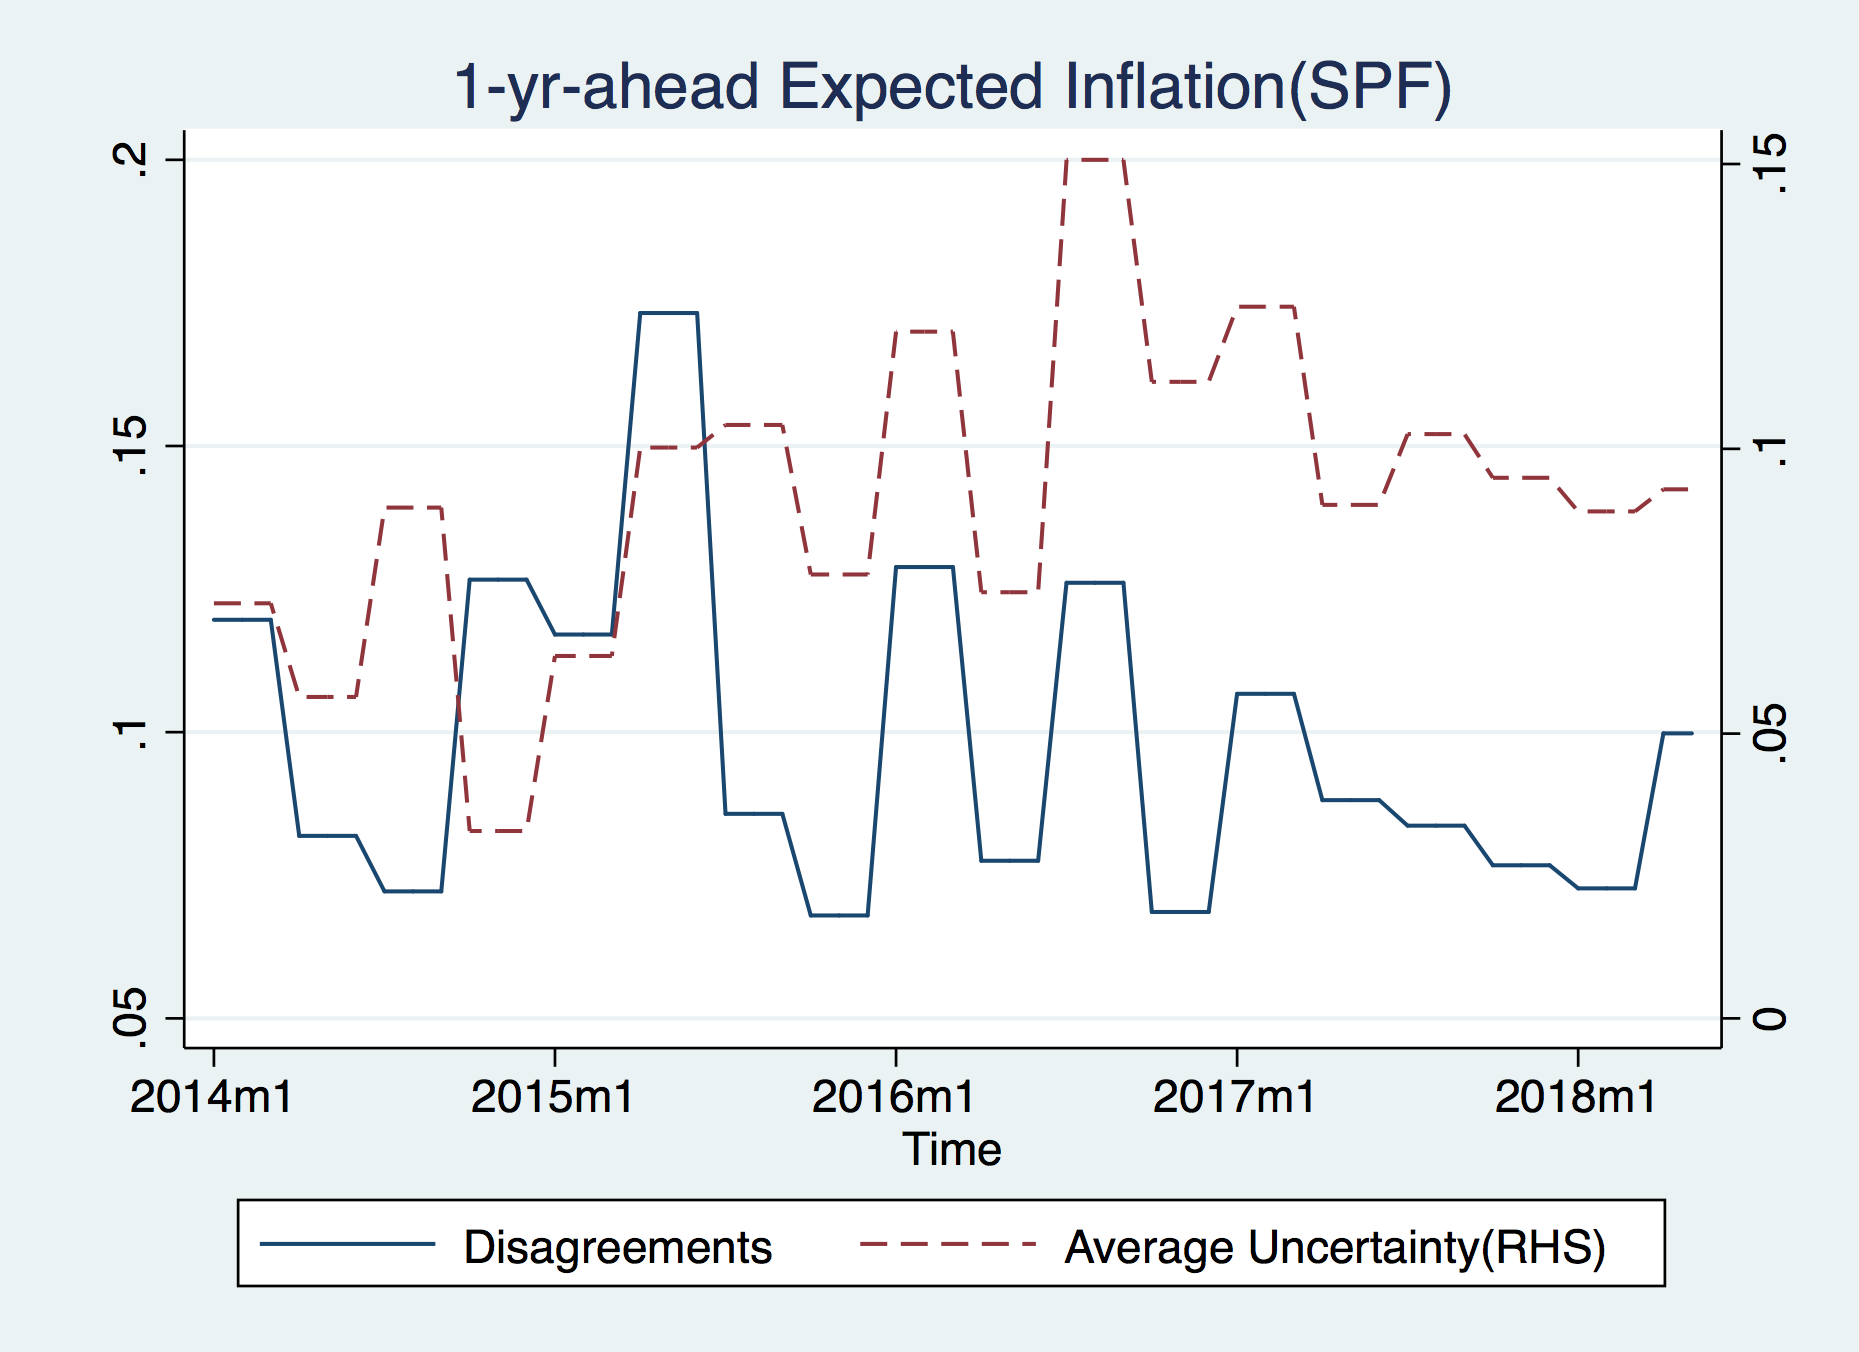
\includegraphics[scale=0.3]{figures/var_disg2.png} 
\end{figure}
\end{frame}


\begin{frame}{Population moments: forecast and realization}
\begin{figure}
	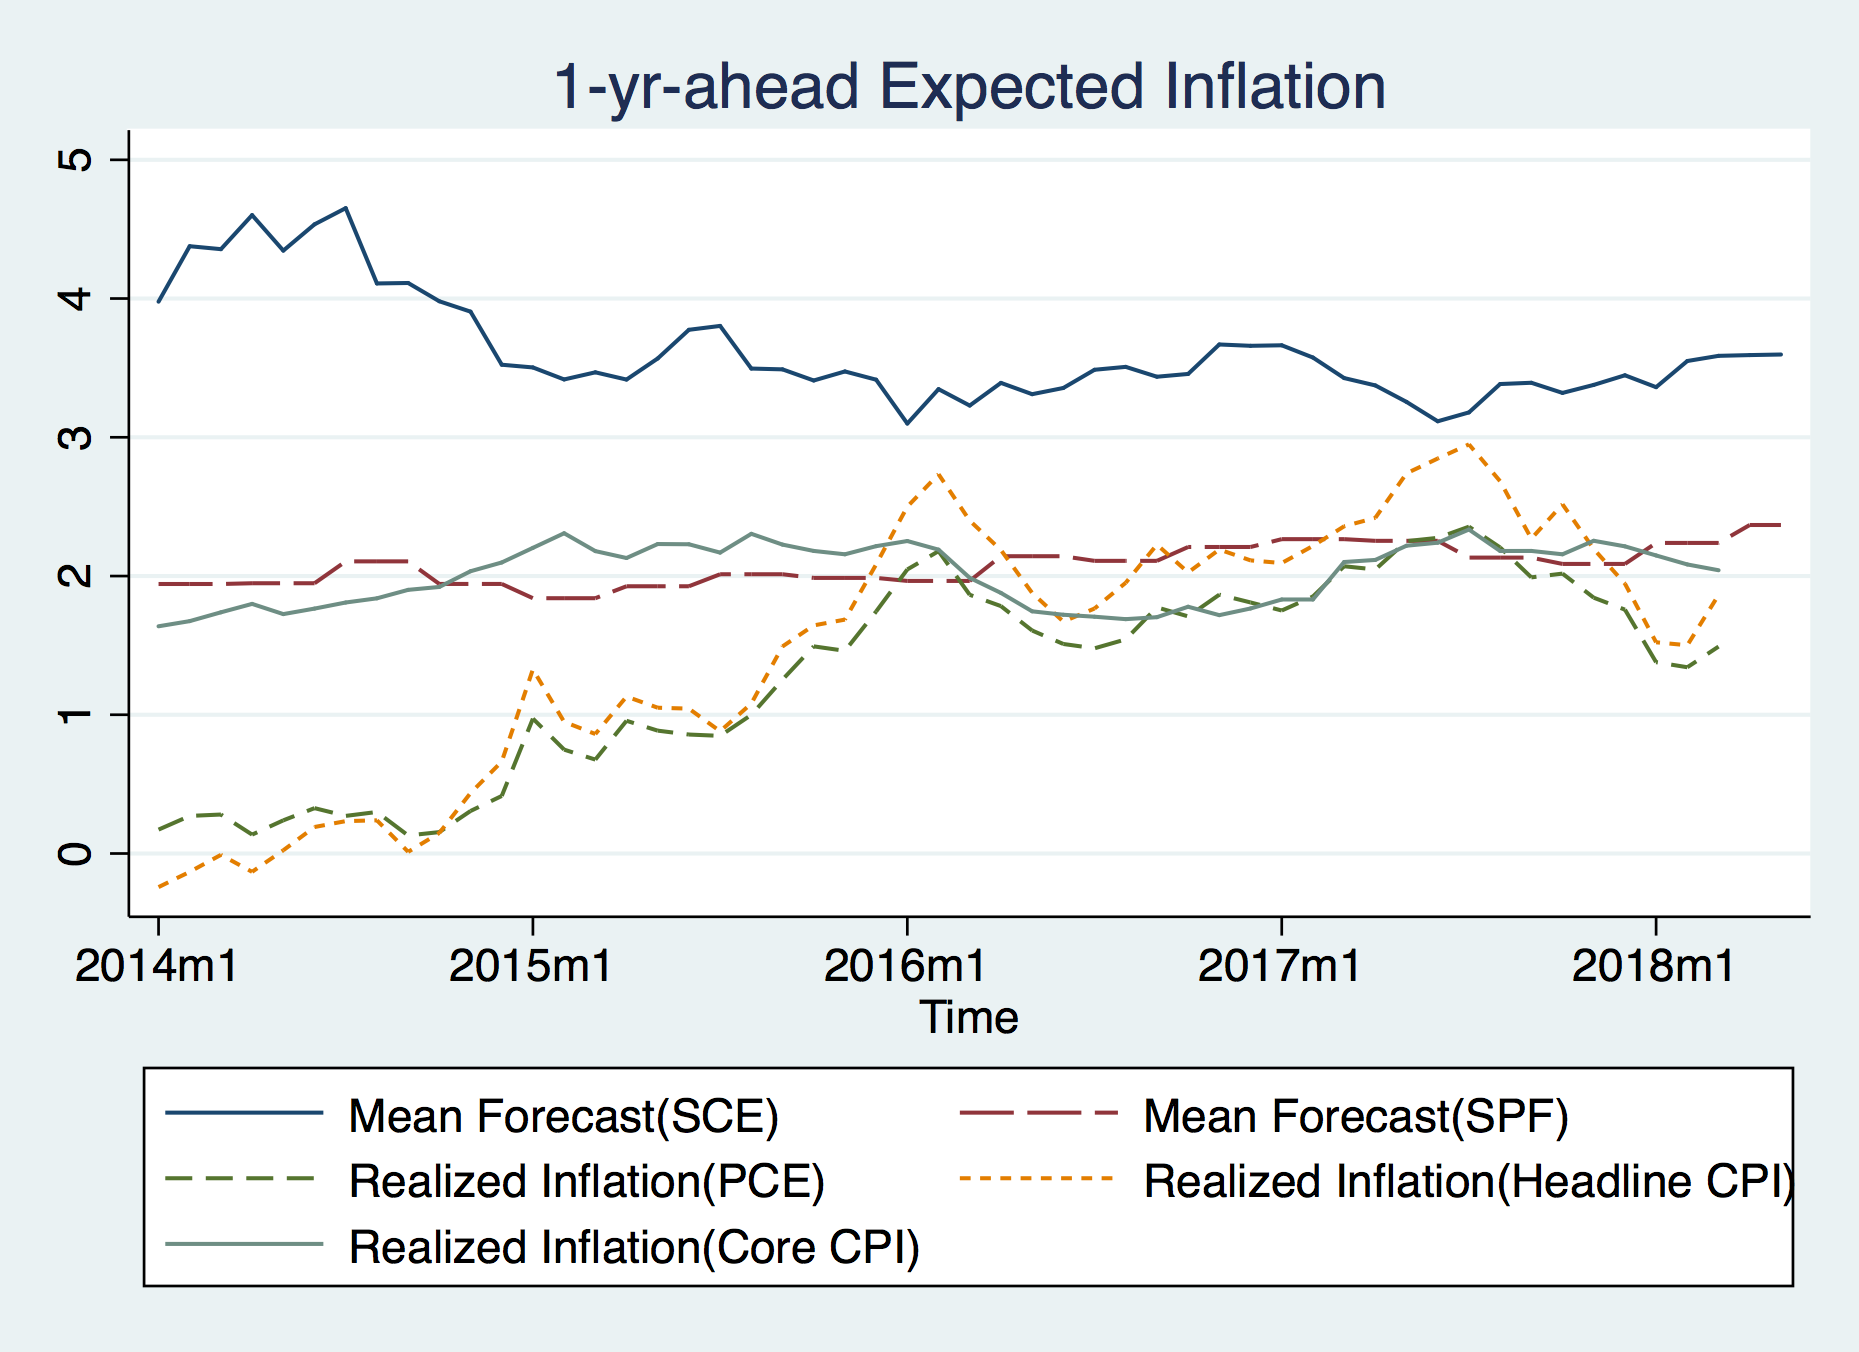
\includegraphics[scale=0.3]{figures/mean_true.png} 
\end{figure}
\end{frame}

\section{Empirical Results}


\begin{frame}{Empirical execution}

\begin{itemize}

\item \textbf{Density Estimation}: generalized beta estimation, \cite{engelberg2009comparing}
 \item \textbf{Identification of Shocks}: following \cite{coibion2012can} and monetary policy shocks. 
\end{itemize}

\end{frame}

\subsection{Test of Null Hypothesis of Rational Expectation}

\begin{frame}{Test of Rational Expectation}
\begin{table}[tbhp] \centering \adjustbox{max height=\dimexpr\textheight-5.5cm\relax, max width=\textwidth}{
	\begin{tabular}{lllllll}
		\hline 
		& SPFCPI\_FElvl       & SPFPCE\_FElvl & SPFCPI\_Vardiff & SPFPCE\_Vardiff & SPFCPI\_Disgdiff & SPFPCE\_Disgdiff            \\
		\hline 
		L.InfExp\_FE        & 0.941***      & 1.195***        &                 &                  &                  &           \\
		& (0.0840)      & (0.142)         &                 &                  &                  &           \\
		L2.InfExp\_FE       & -0.313**      & -0.625**        &                 &                  &                  &           \\
		& (0.116)       & (0.198)         &                 &                  &                  &           \\
		L3.InfExp\_FE       & 0.114         & 0.0782          &                 &                  &                  &           \\
		& (0.114)       & (0.196)         &                 &                  &                  &           \\
		L4.InfExp\_FE       & -0.137        & -0.0162         &                 &                  &                  &           \\
		& (0.0820)      & (0.131)         &                 &                  &                  &           \\
		L.InfExp\_Var\_ch   &               &                 & -0.855***       & -0.565**         &                  &           \\
		&               &                 & (0.189)         & (0.162)          &                  &           \\
		L2.InfExp\_Var\_ch  &               &                 & -0.780**        & -0.452*          &                  &           \\
		&               &                 & (0.220)         & (0.186)          &                  &           \\
		L3.InfExp\_Var\_ch  &               &                 & -0.556*         & -0.429*          &                  &           \\
		&               &                 & (0.219)         & (0.189)          &                  &           \\
		L4.InfExp\_Var\_ch  &               &                 & -0.167          & 0.00385          &                  &           \\
		&               &                 & (0.188)         & (0.172)          &                  &           \\
		L.InfExp\_Disg\_ch  &               &                 &                 &                  & -0.571***        & -0.640*** \\
		&               &                 &                 &                  & (0.0699)         & (0.127)   \\
		L2.InfExp\_Disg\_ch &               &                 &                 &                  & -0.376***        & -0.0944   \\
		&               &                 &                 &                  & (0.0764)         & (0.141)   \\
		L3.InfExp\_Disg\_ch &               &                 &                 &                  & -0.0455          & 0.180     \\
		&               &                 &                 &                  & (0.0661)         & (0.138)   \\
		L4.InfExp\_Disg\_ch &               &                 &                 &                  & -0.110*          & -0.0364   \\
		&               &                 &                 &                  & (0.0479)         & (0.123)   \\
		\hline 
		N                   & 143           & 41              & 44              & 44               & 146              & 44        \\
		R-sq                & 0.593         & 0.750           & 0.384           & 0.322            & 0.356            & 0.496    \\
		\hline 
	\end{tabular}
}
\end{table}
\end{frame}


\begin{frame}{Inflation shocks}

\begin{figure}
	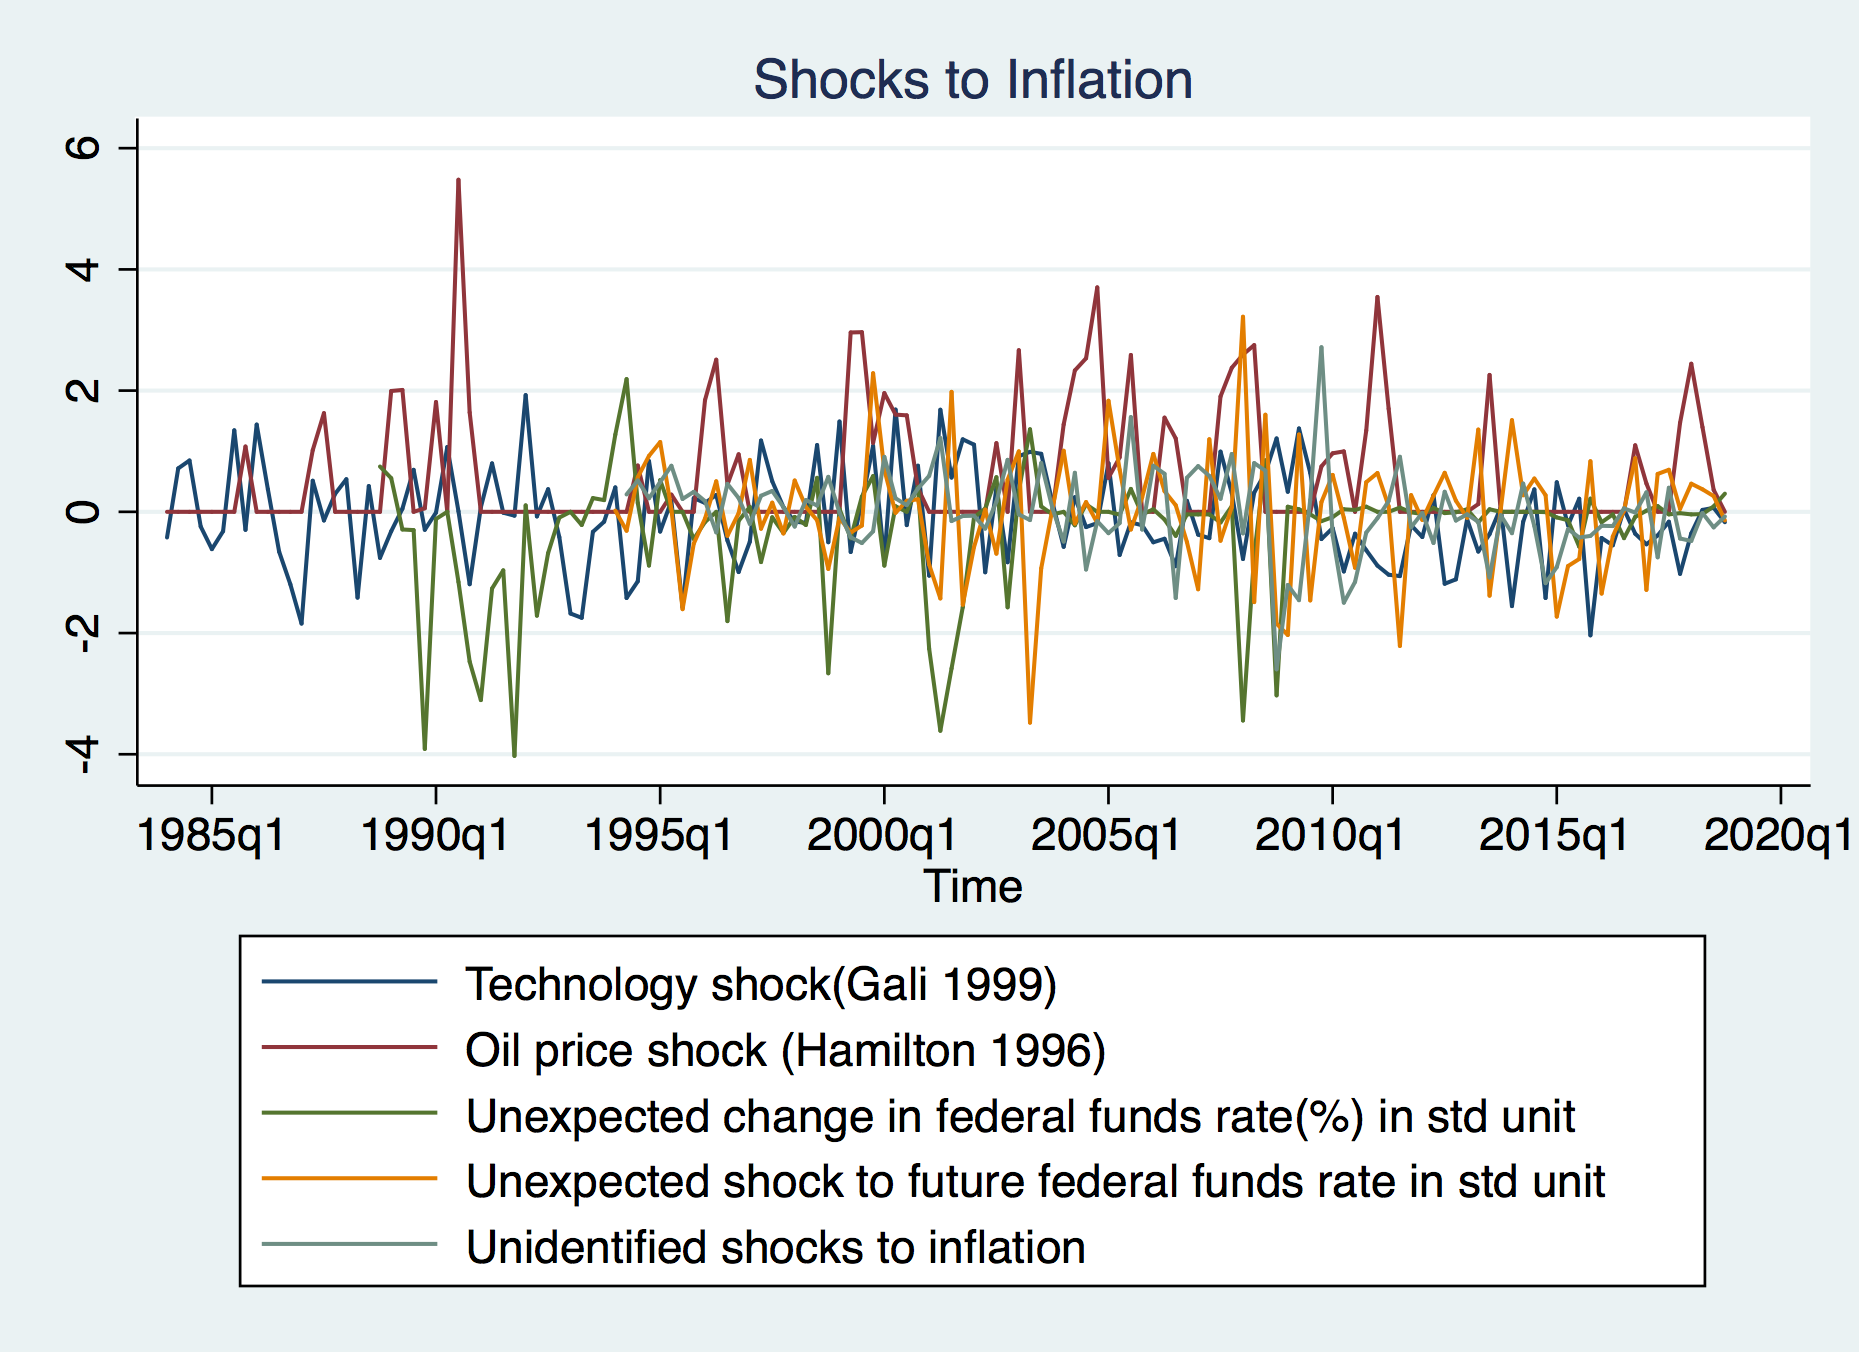
\includegraphics[scale=0.3]{figures/inf_shocksQ.png} 
\end{figure}

\end{frame}

\begin{frame}{Results from \cite{coibion2012can}}

\begin{figure}
	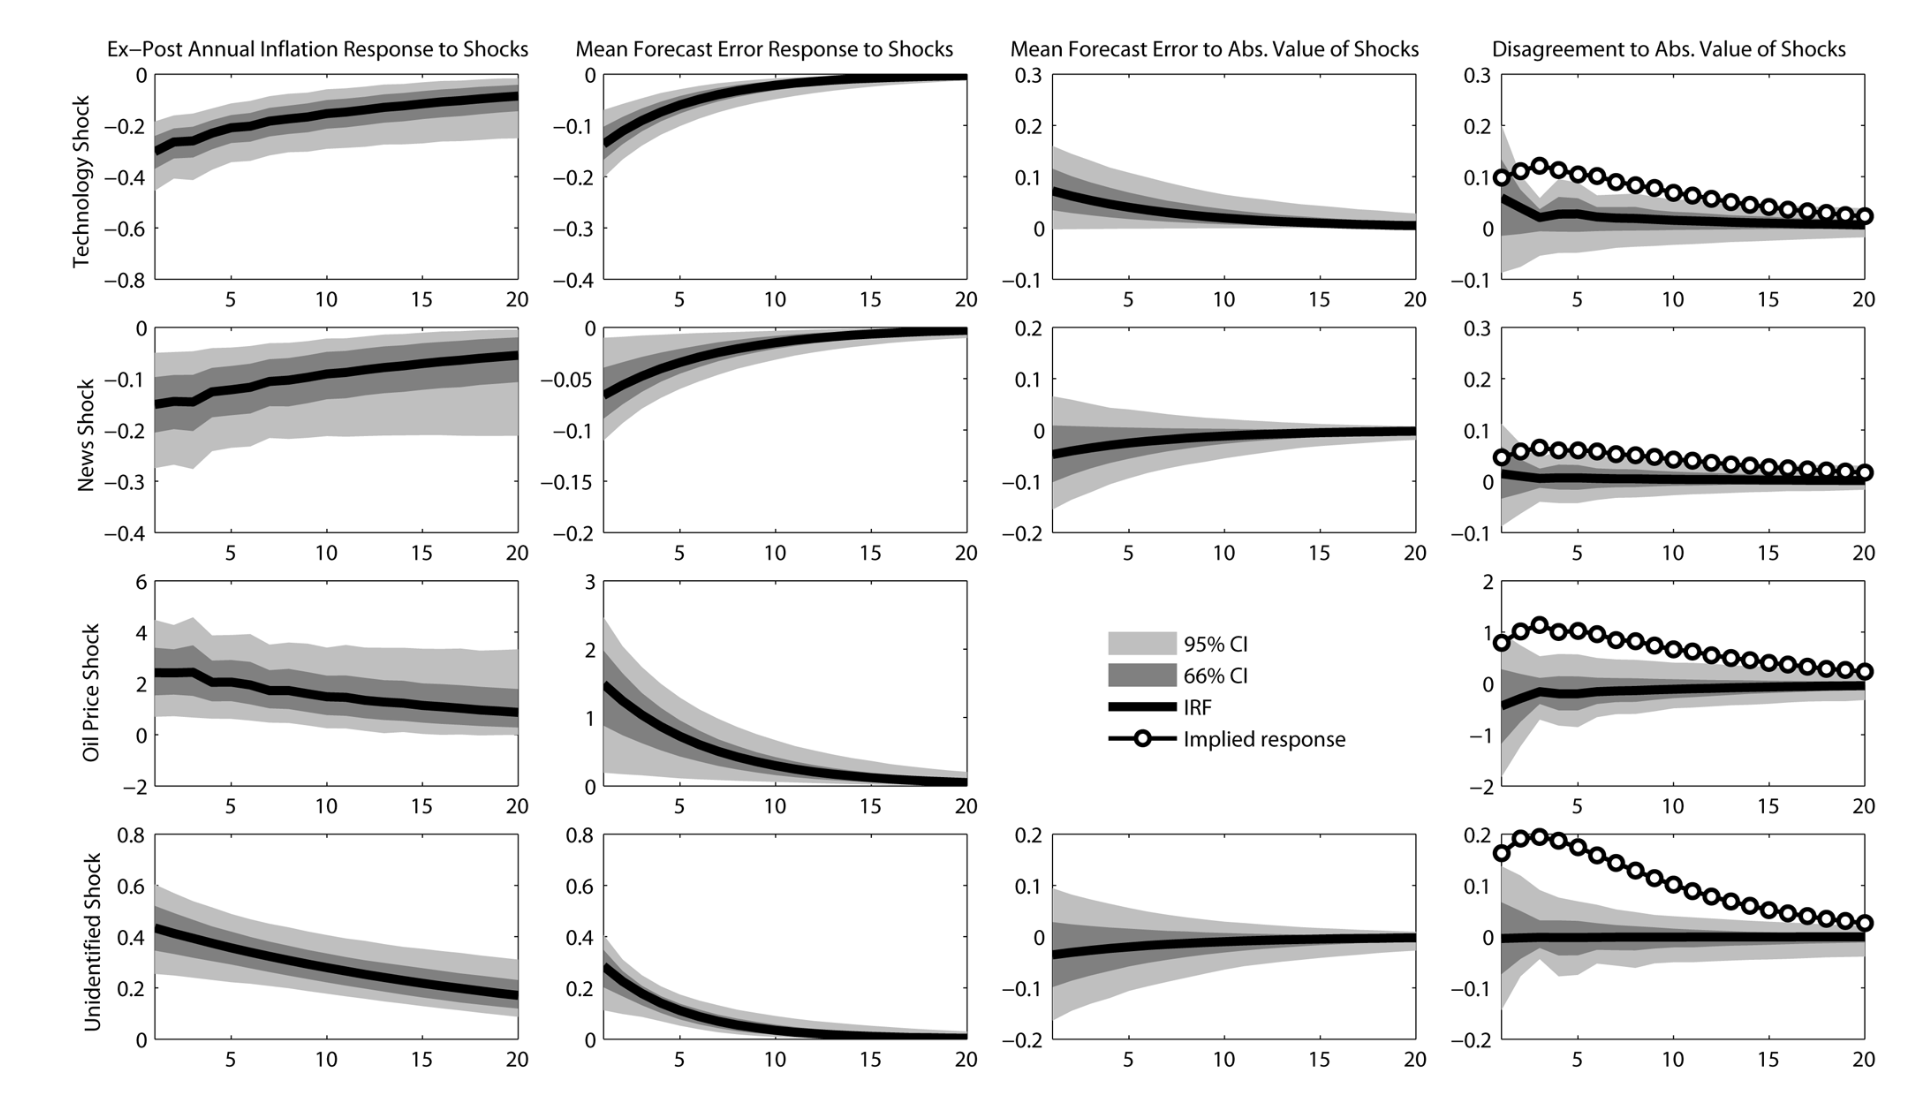
\includegraphics[scale=0.3]{figures/RigidityJPEFigure2.png} 
\end{figure}

\end{frame}

\begin{frame}{Inflation IR to  shocks exluding monetary policy}

\begin{figure}
	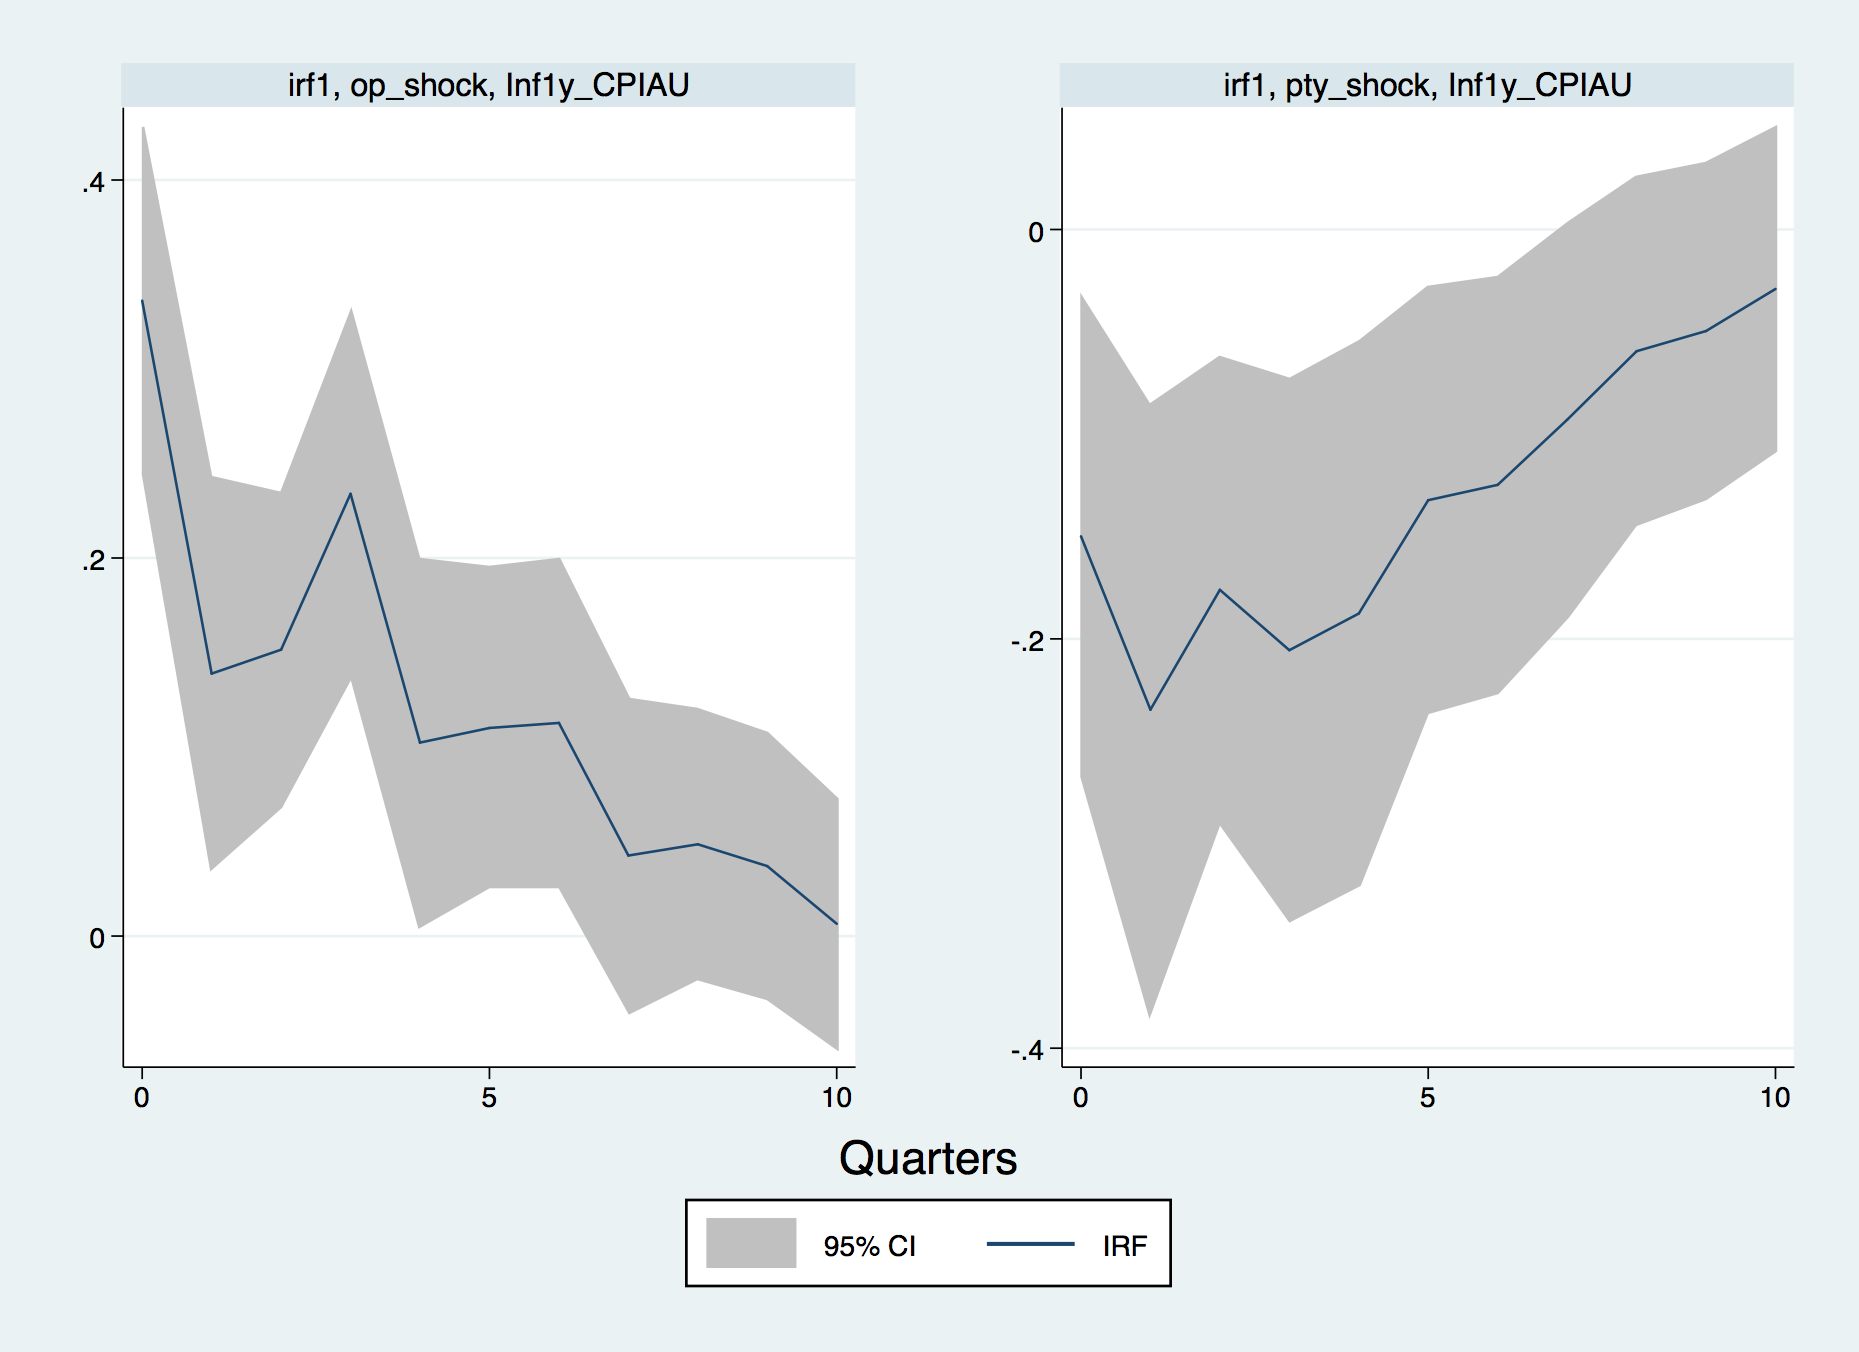
\includegraphics[scale=0.3]{figures/CPIAU_ashocks_nmp.png} 
\end{figure}

\end{frame}


\begin{frame}{Inflation IR to  shocks including monetary policy}

\begin{figure}
	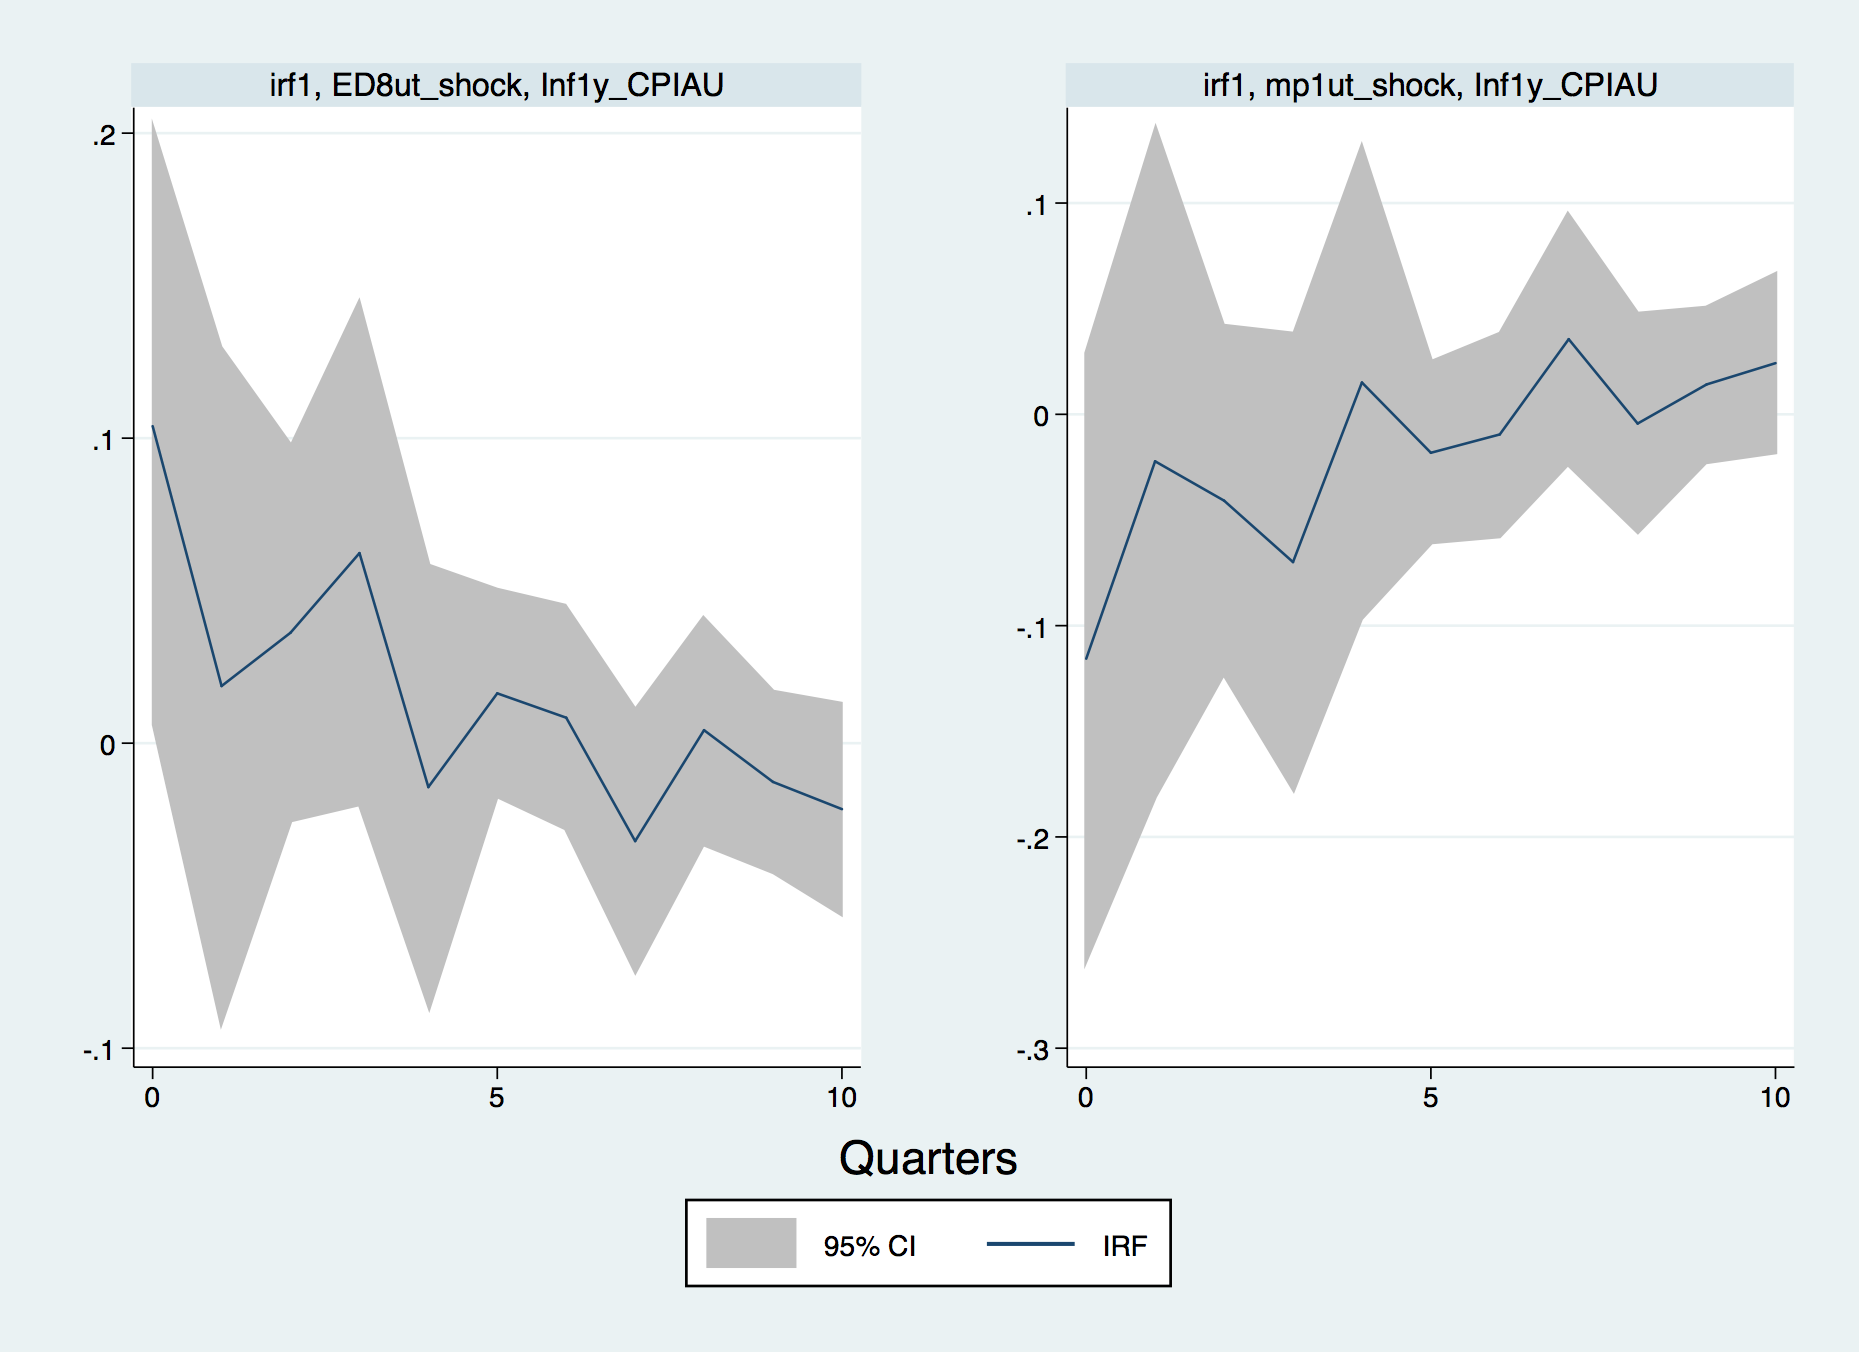
\includegraphics[scale=0.3]{figures/CPIAU_ashocks.png} 
\end{figure}

\end{frame}


\begin{frame}{Inflation IR to  shocks excluding monetary policy}

\begin{figure}
	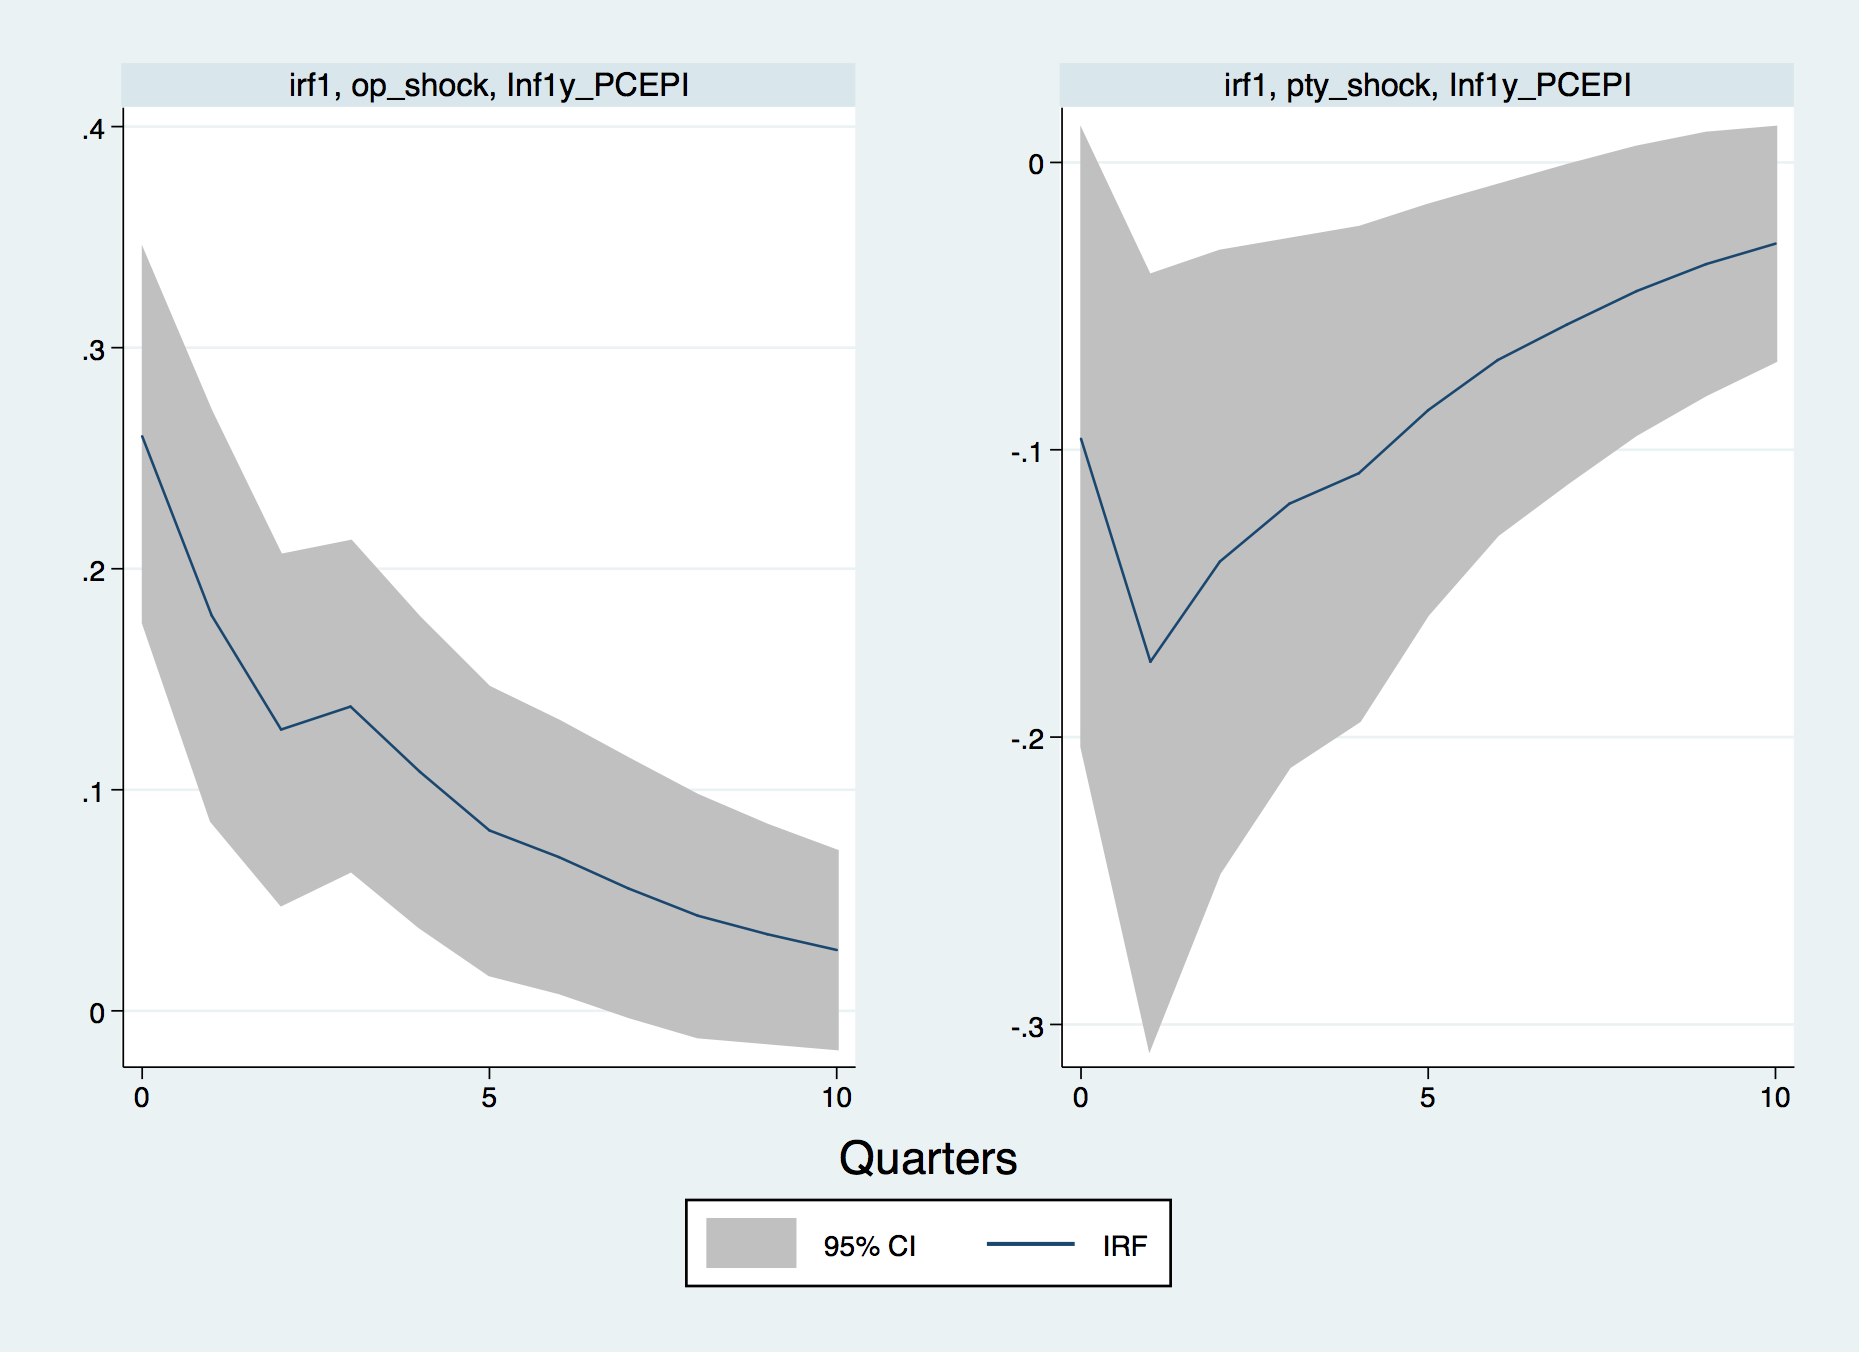
\includegraphics[scale=0.3]{figures/PCEPI_ashocks_nmp.png} 
\end{figure}

\end{frame}



\begin{frame}{Inflation IR to  shocks including monetary policy}

\begin{figure}
	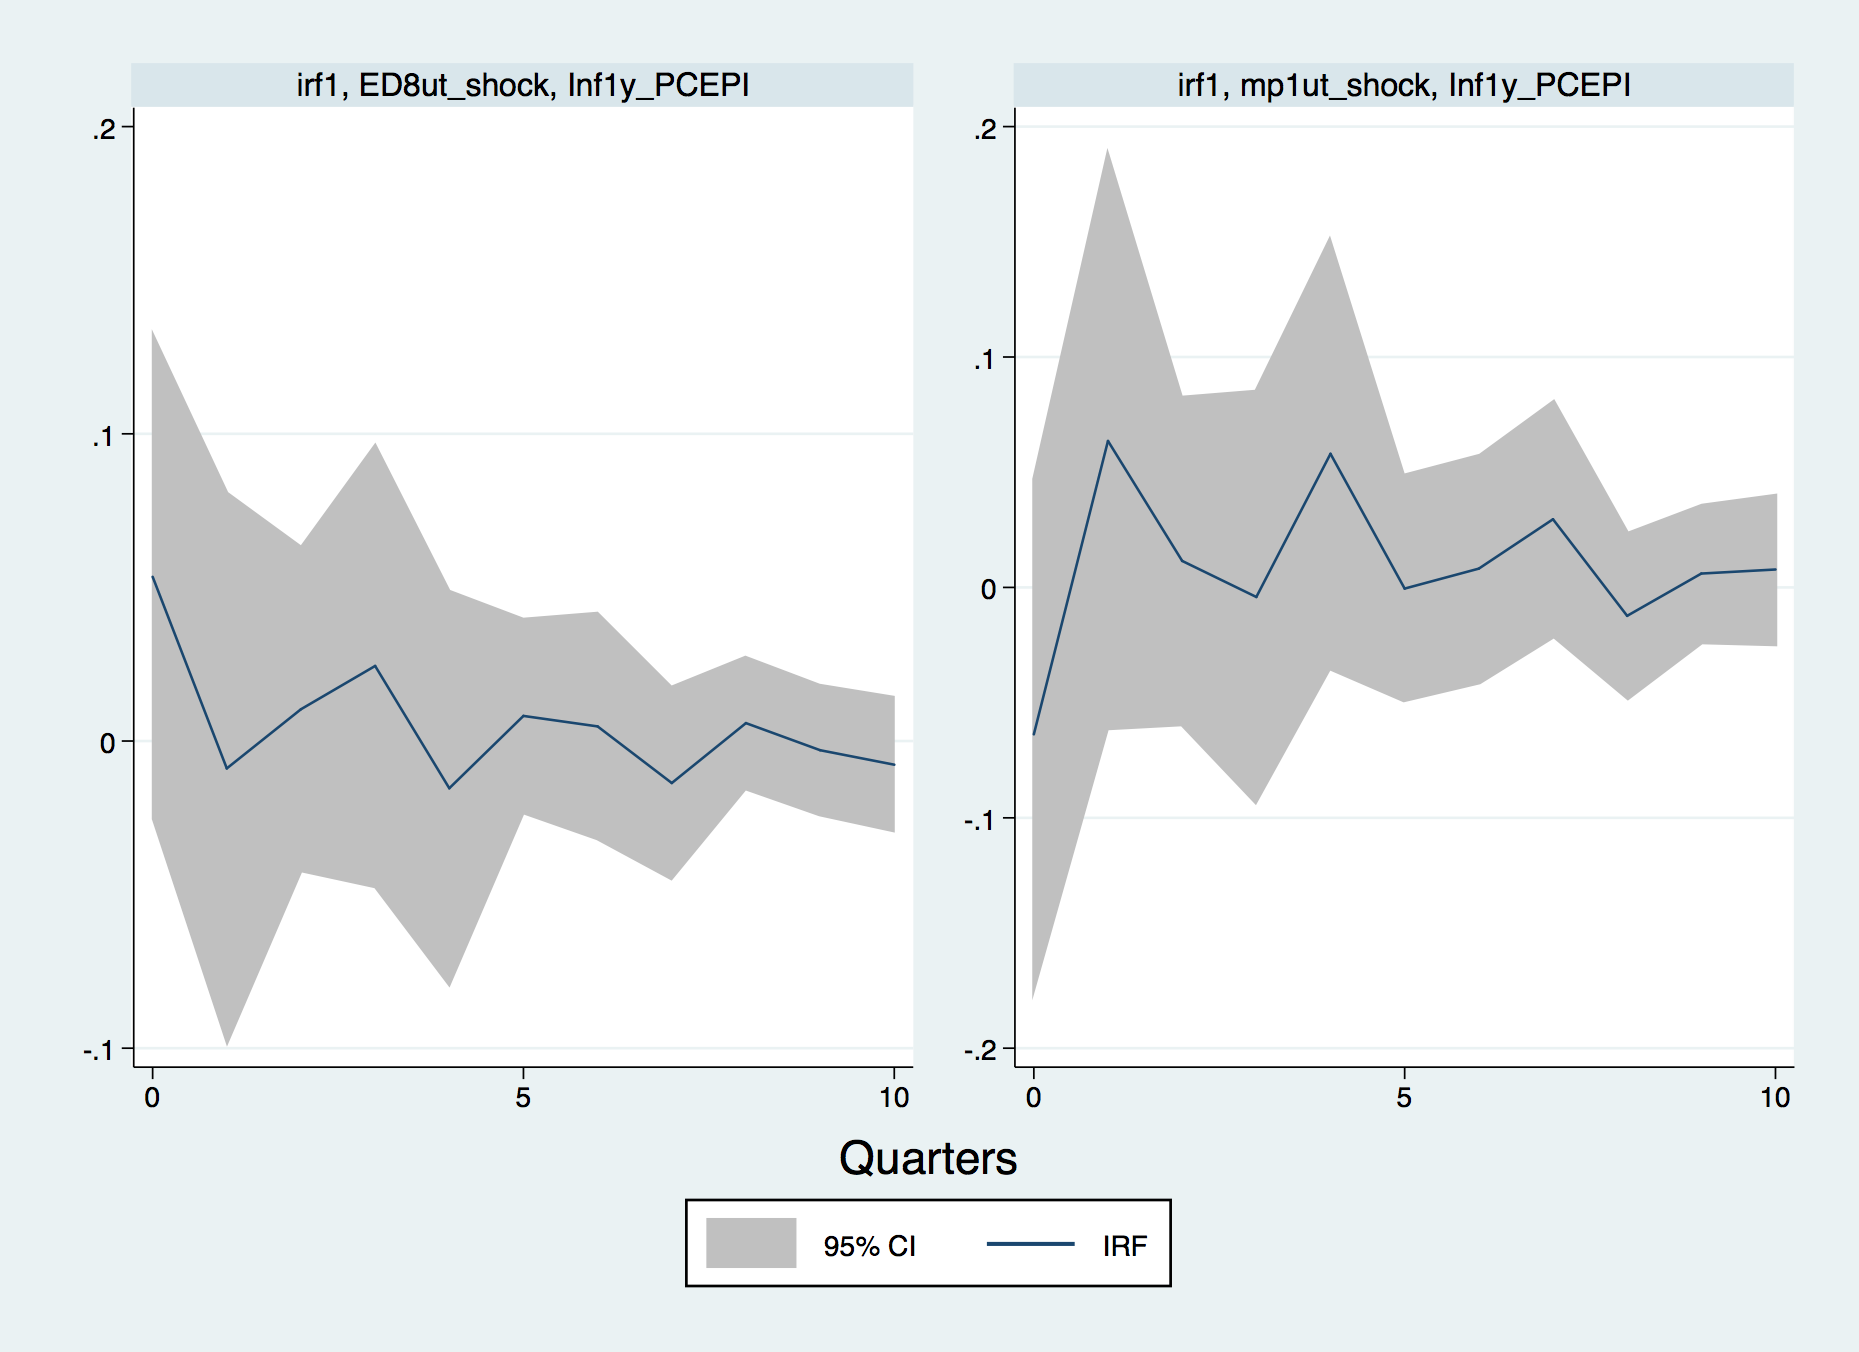
\includegraphics[scale=0.3]{figures/PCEPI_ashocks.png} 
\end{figure}

\end{frame}

\subsection{Benchmark Results from Professional Forecasters }

\begin{frame}{Forecasting errors IR to  shocks excluding monetary policy}

\begin{figure}
	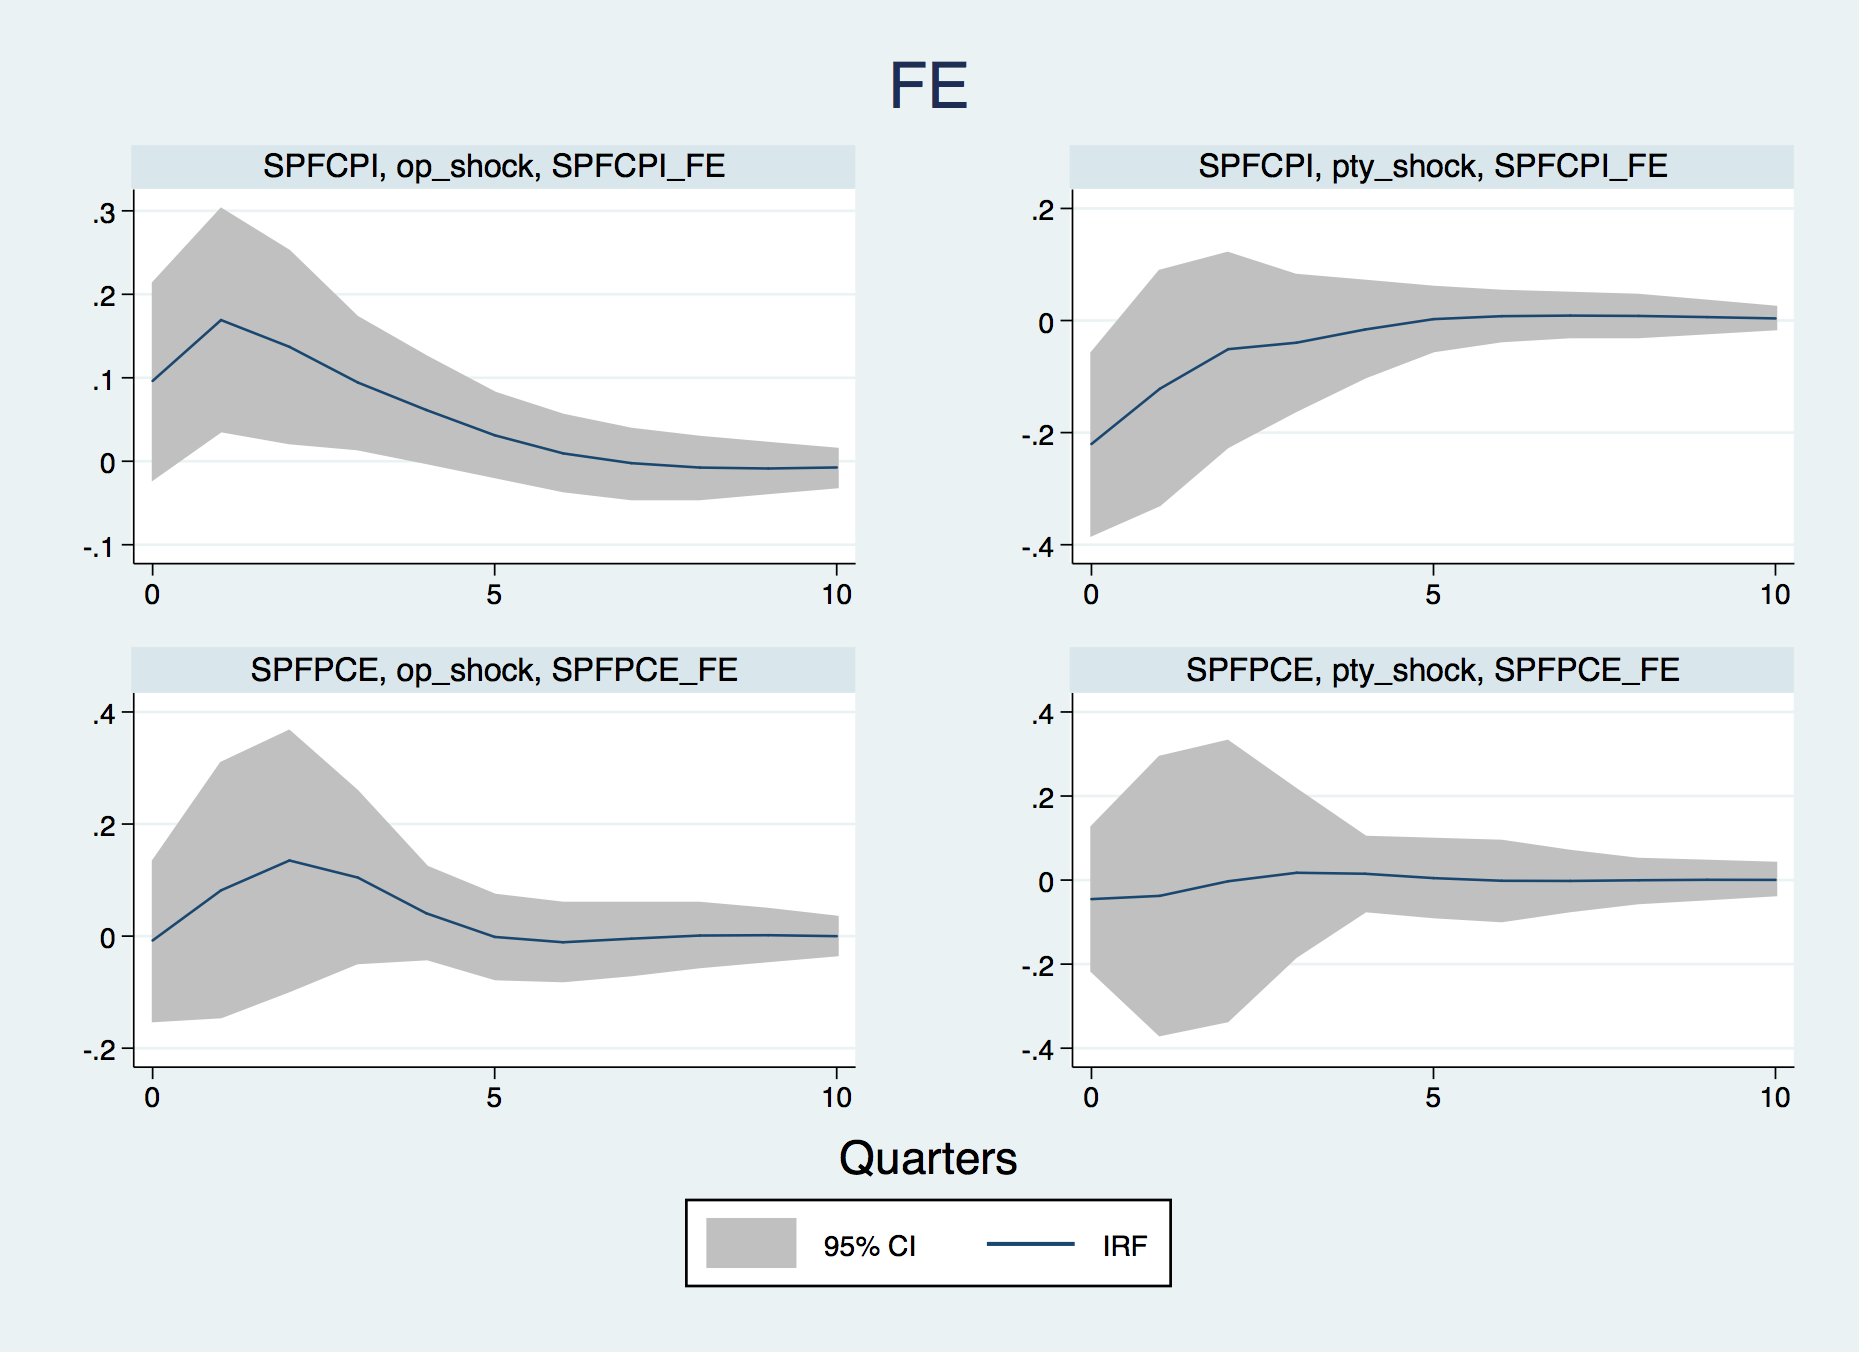
\includegraphics[scale=0.3]{figures/SPFFE_ashocks_nmp.png} 
\end{figure}

\end{frame}


\begin{frame}{Forecasting errors IR to monetary policy shocks}

\begin{figure}
	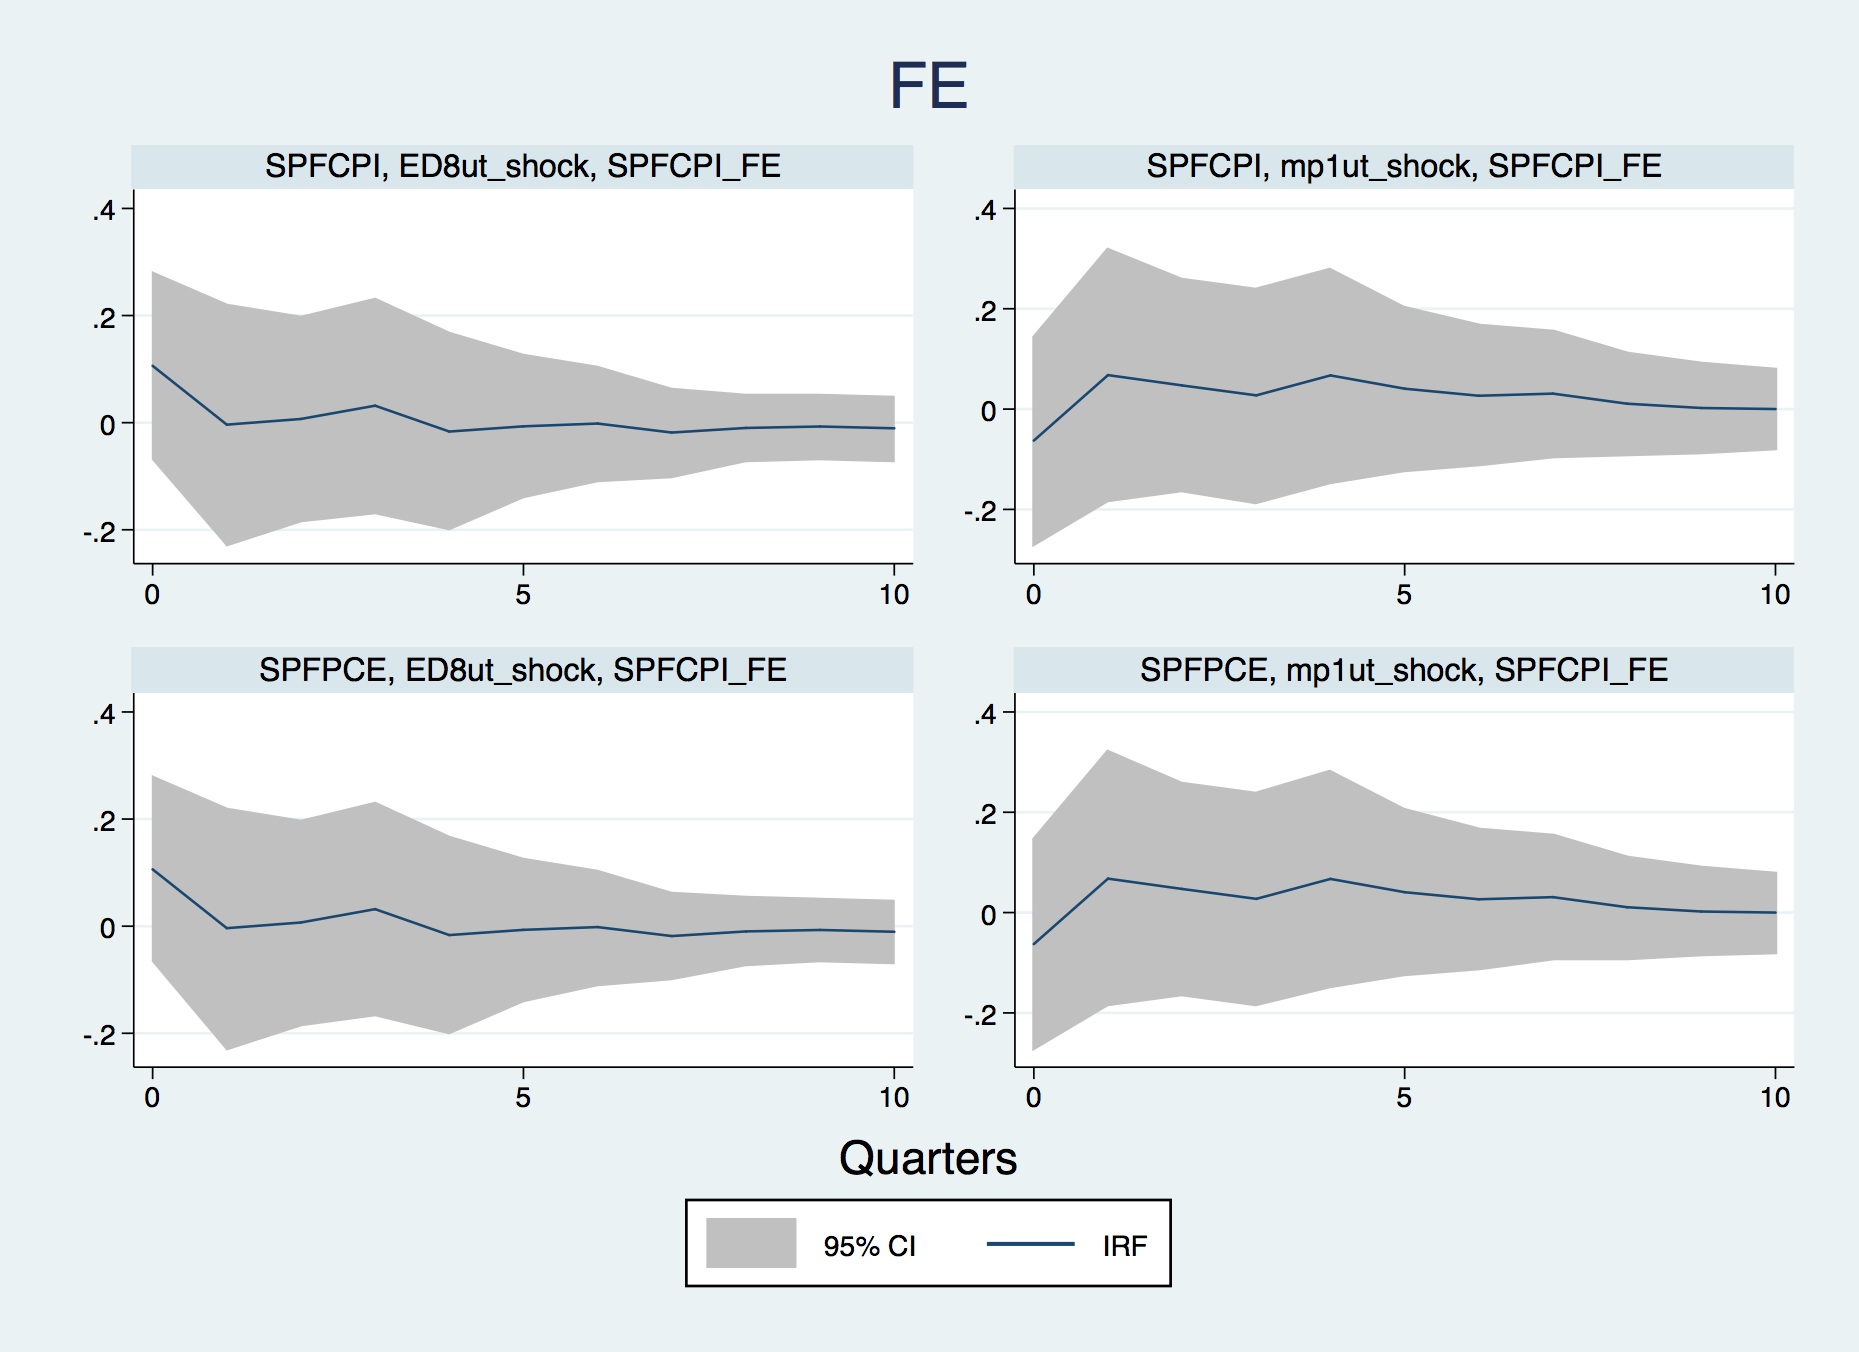
\includegraphics[scale=0.3]{figures/SPFFE_ashocks.png} 
\end{figure}

\end{frame}


\begin{frame}{Disagreements IR to shocks excluding monetary policy}

\begin{figure}
	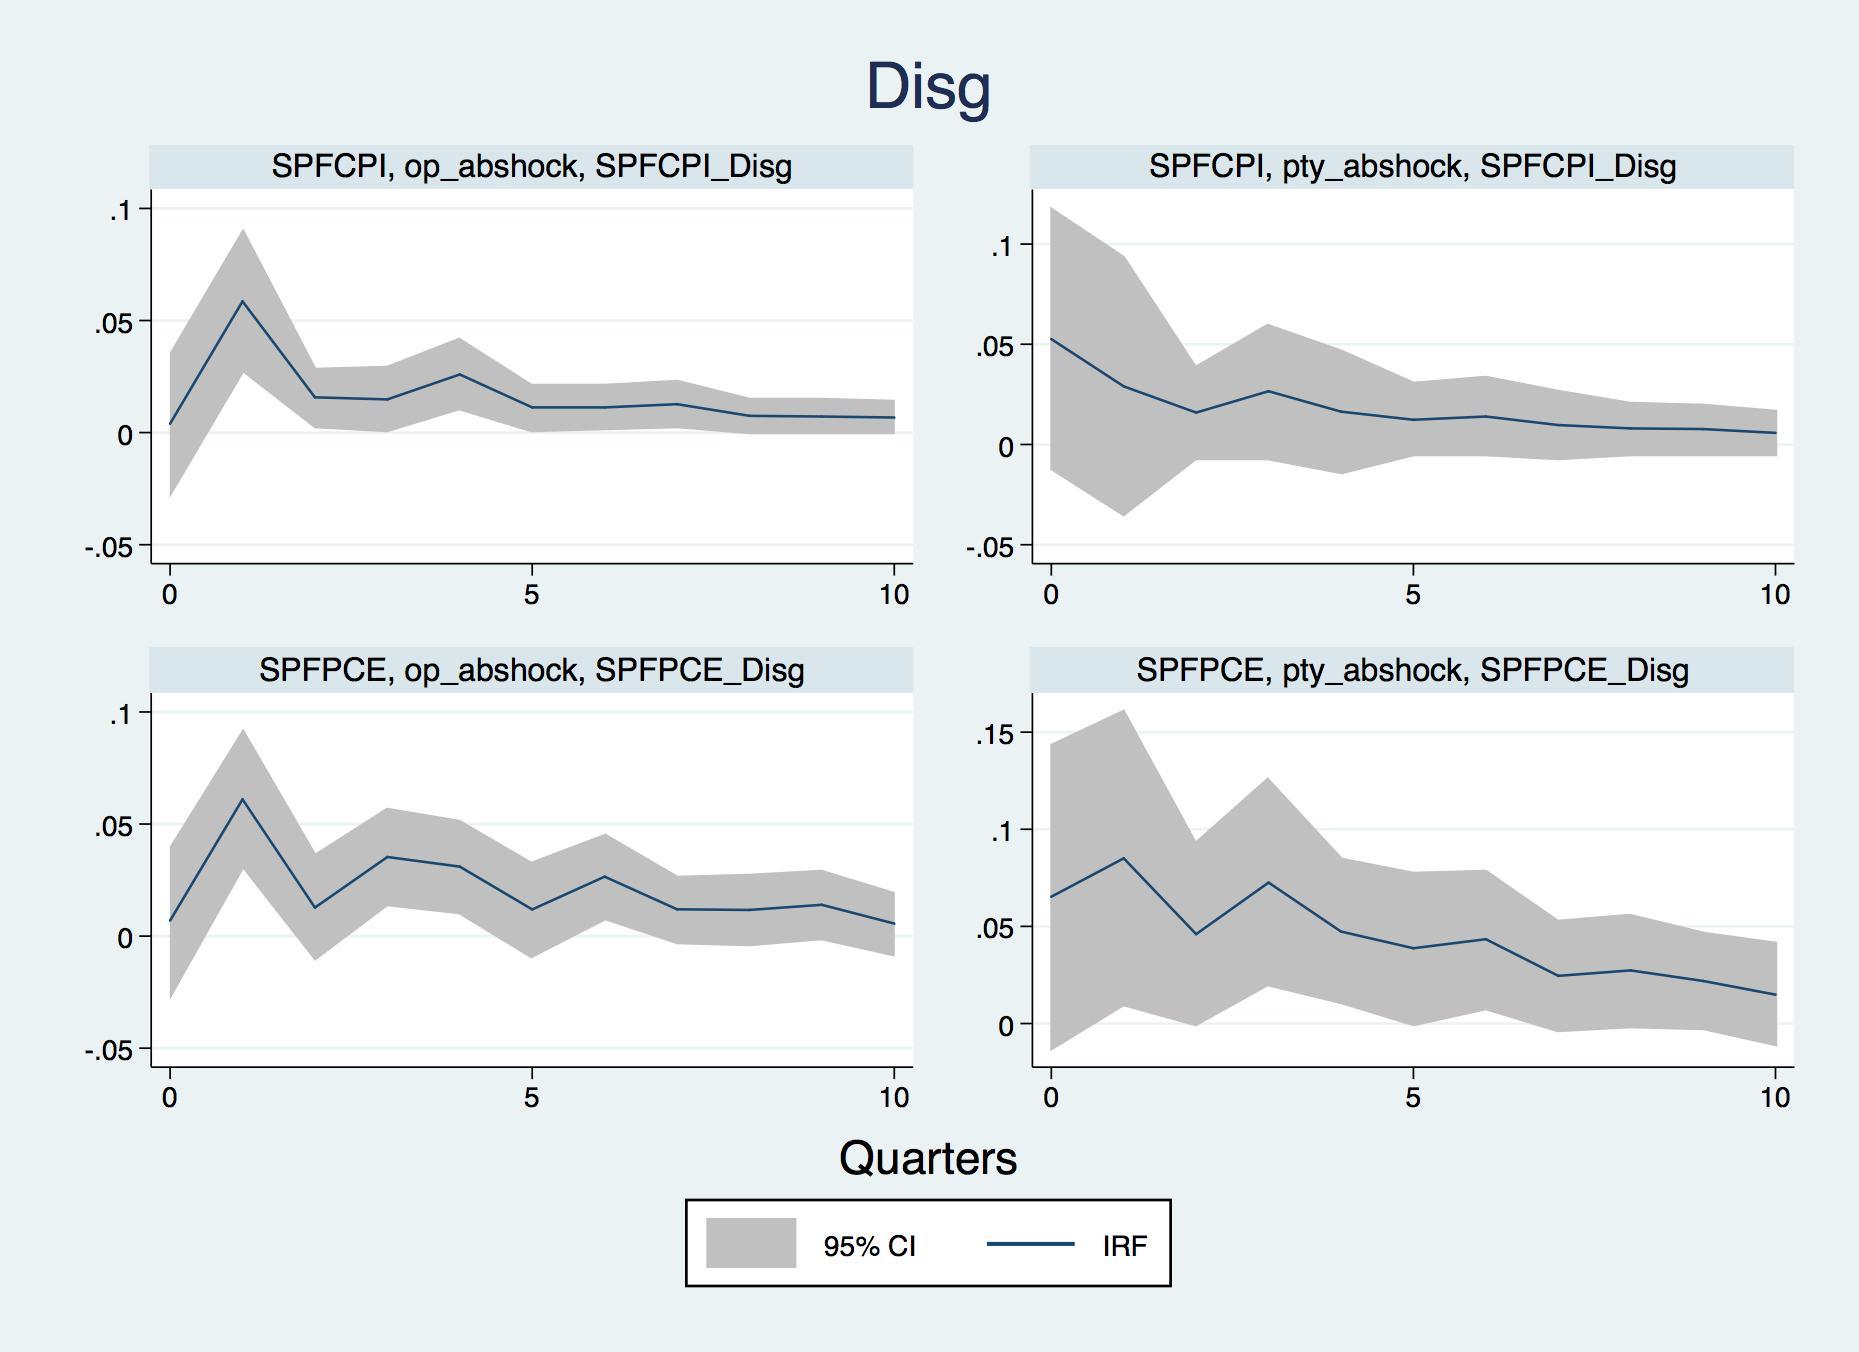
\includegraphics[scale=0.3]{figures/SPFDisg_ab_ashocks_nmp.png} 
\end{figure}

\end{frame}


\begin{frame}{Disagreements IR to  monetary policy shocks}

\begin{figure}
	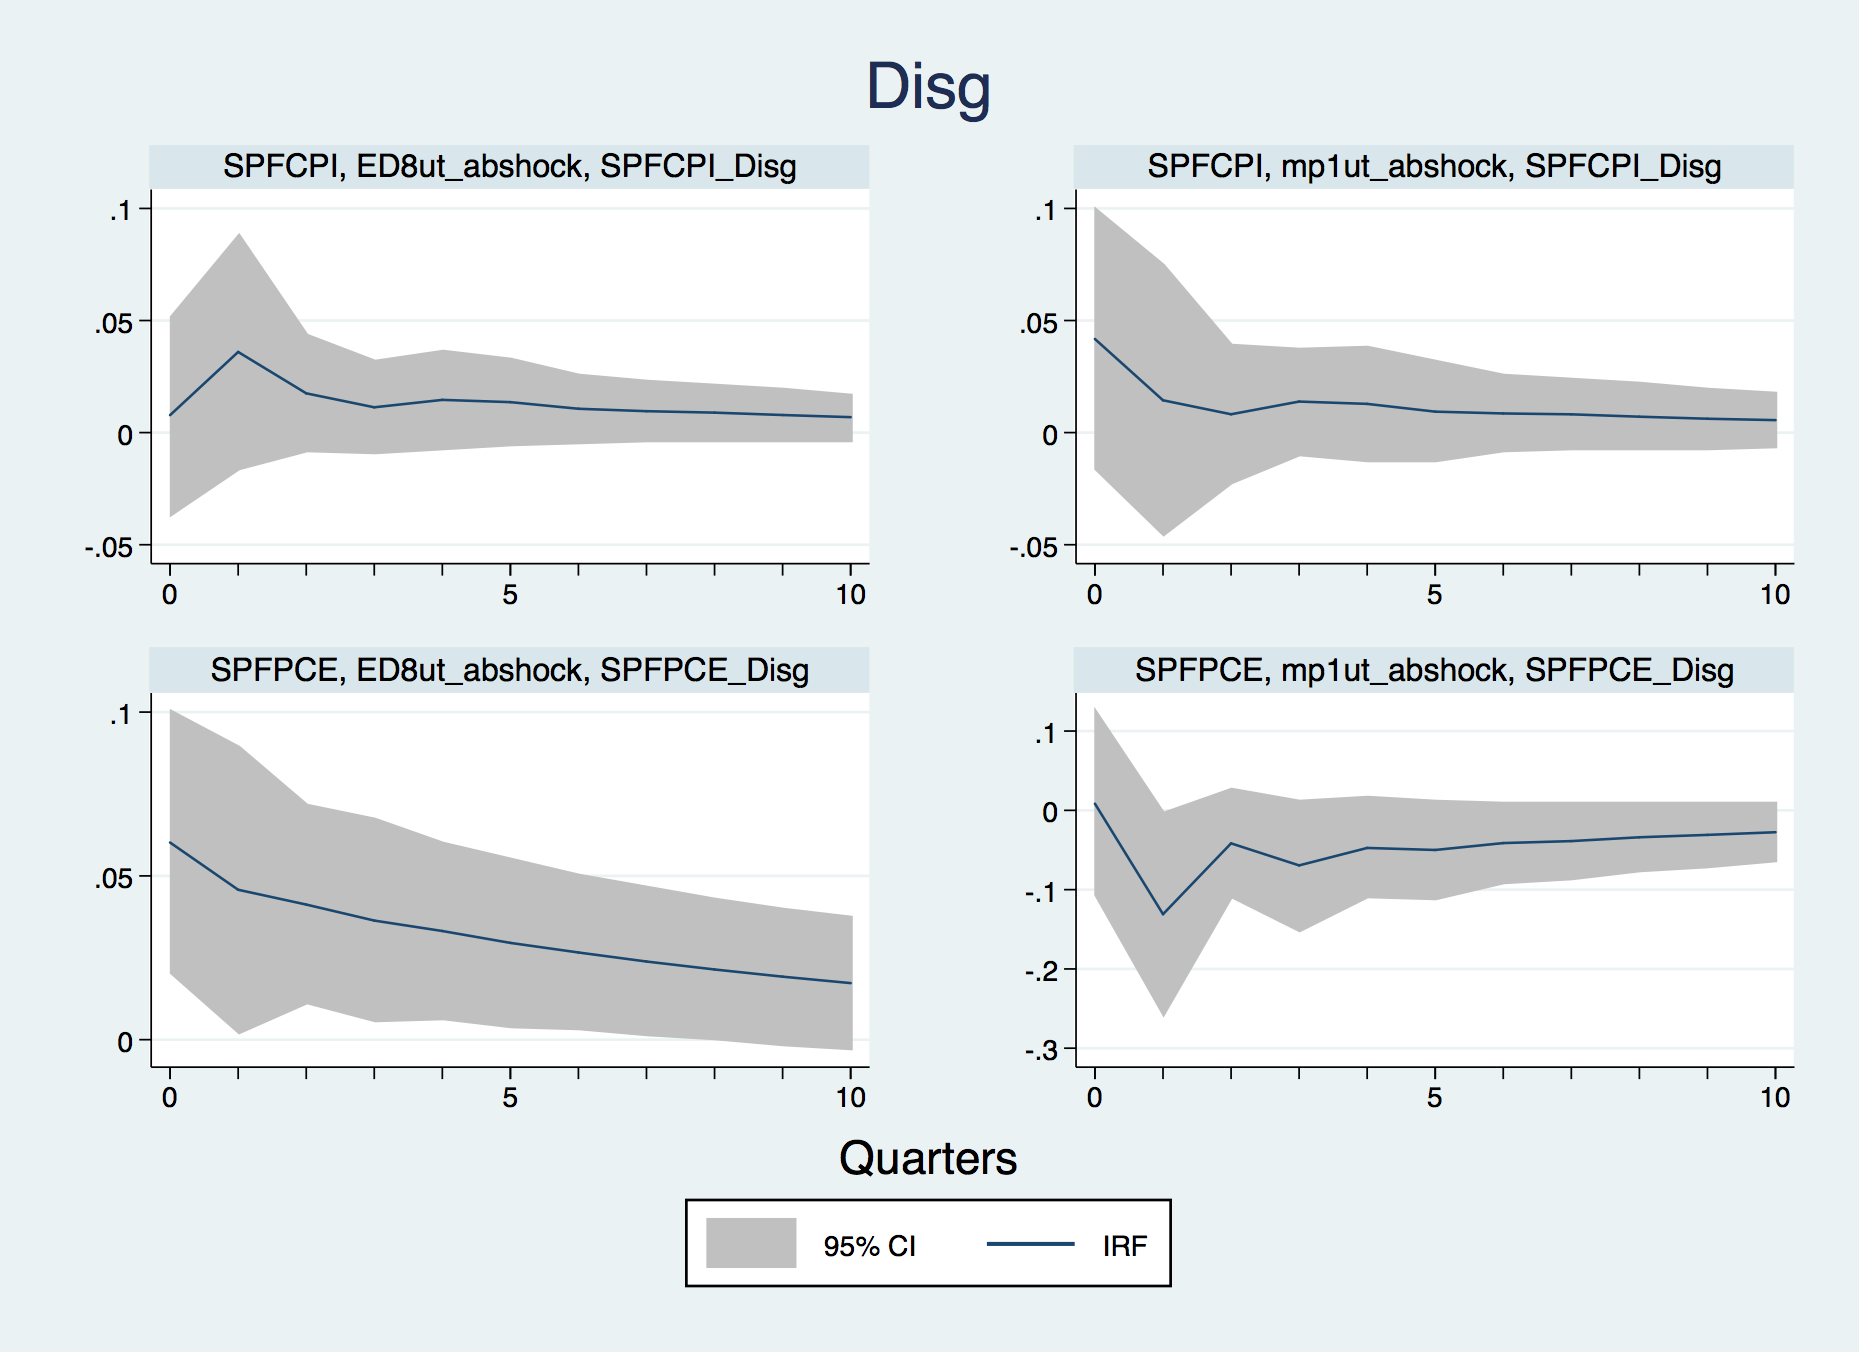
\includegraphics[scale=0.3]{figures/SPFDisg_ab_ashocks.png} 
\end{figure}

\end{frame}


\begin{frame}{Uncertainty IR to shocks excluding monetary policy}

\begin{figure}
	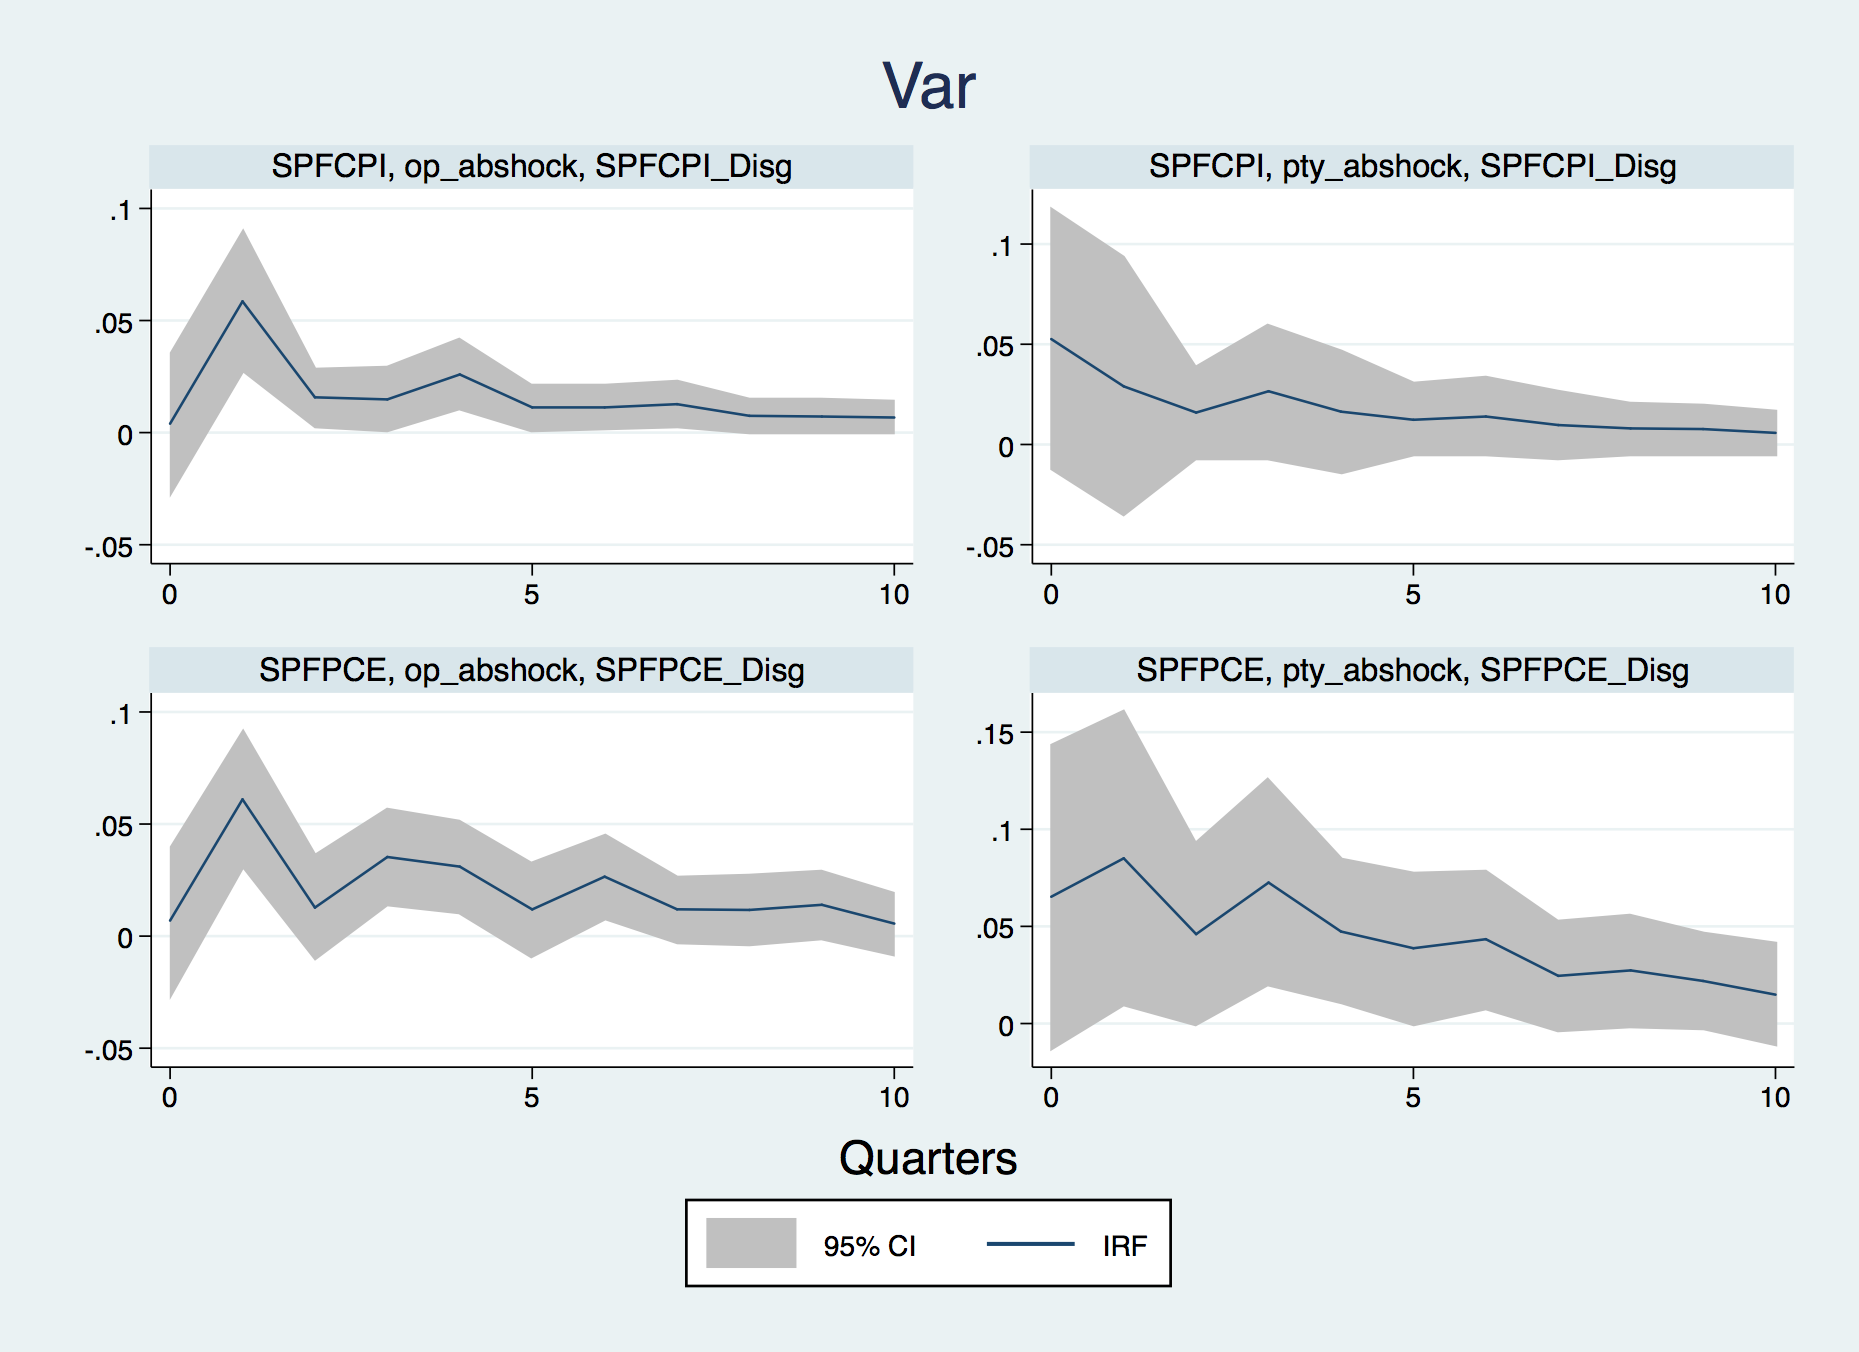
\includegraphics[scale=0.3]{figures/SPFVar_ab_ashocks_nmp.png} 
\end{figure}

\end{frame}


\begin{frame}{Uncertainty IR to monetary policy shocks}

\begin{figure}
	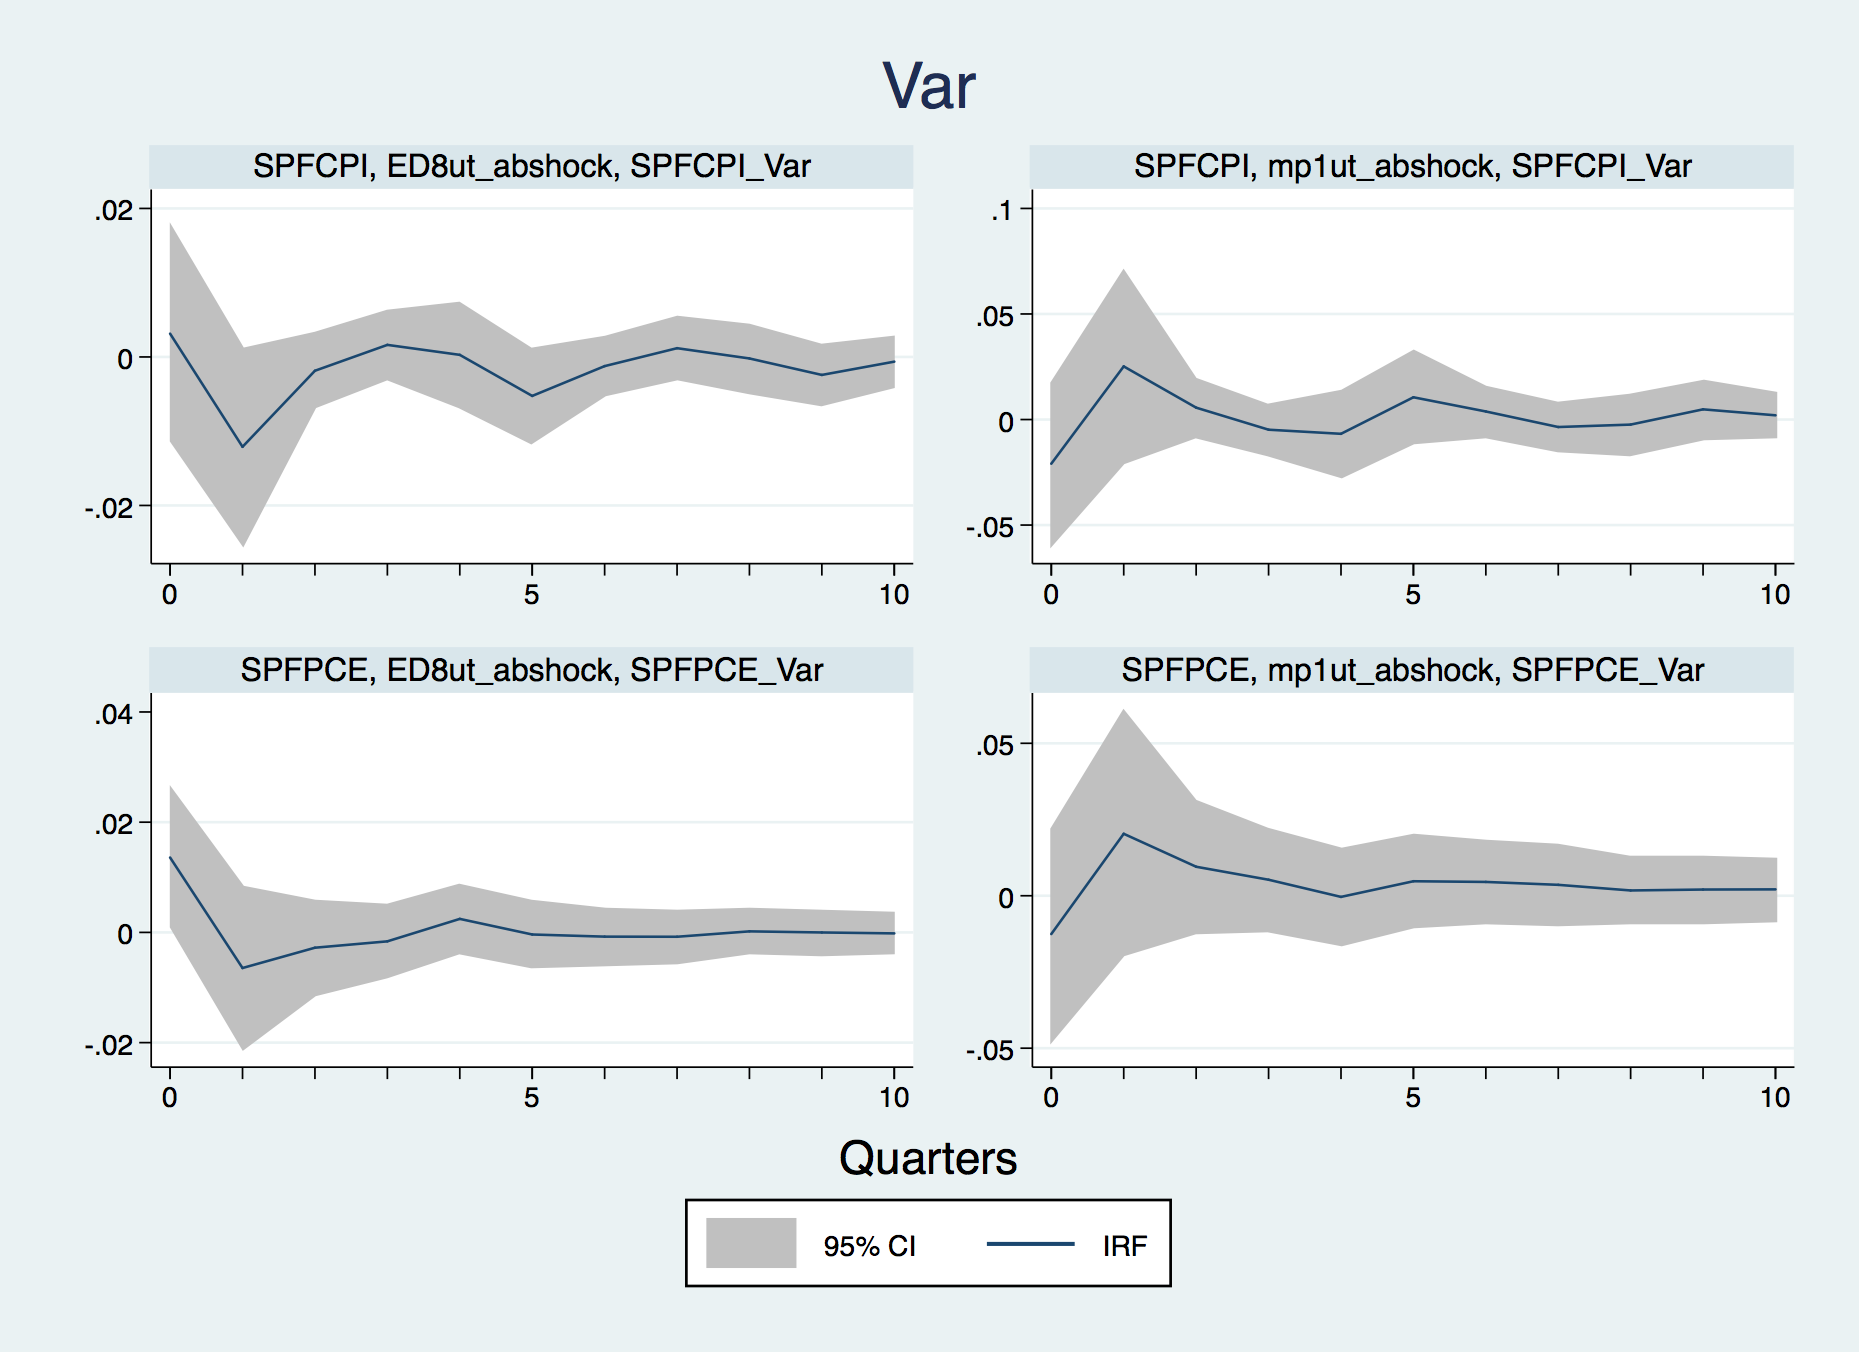
\includegraphics[scale=0.3]{figures/SPFVar_ab_ashocks.png} 
\end{figure}

\end{frame}


\bibliographystyle{apalike}
\bibliography{ExpSlides}

\section{Appendix}




\begin{frame}{Sticky Expectation: individual}

For a non-updater since $t-\tau$ ($\tau=0$ for updater),
\begin{itemize}
\item \textbf{Mean} $$E_{i,t}(y_{t+h}|y_{t-\tau}) = \rho^{h+\tau} y_{t-\tau}$$  
\item \textbf{Forecast Error} $$FE_{i,t+h|t} = \underbrace{\sum^{h+\tau}_{s=0} \rho^s \omega_{t+h-s}}_{\substack{\text{weighted sum of} \\ \text{future realized shocks}} }$$
\item \textcolor{blue}{\textbf{Variance}} $$Var_{i,t}(y_{t+h}|y_{t-\tau}) = \sum^{h+\tau}_{s=0}\rho^{2s} \sigma^2_{\omega}$$	
\end{itemize}

\end{frame}


\begin{frame}{Sticky Expectation: individual}

$$\text{updater: } \quad \Delta Var_{i,t}(y_{t+h}|y_t)= \sum^{\tau}_{s=0} \rho^{2s}\sigma^2_{\omega}$$
$$\text{non-updater: }  \Delta Var_{i,t|t-\tau-1}(y_{t+h}|y_{t-\tau-1})  = \sigma^2_{\omega}$$


\begin{enumerate}
\item Change in expectation(and variance) depends on if update or not 
\item Cannot observe systematically sluggish response to shocks at individual level 
\end{enumerate}

\end{frame}



\begin{frame}{Sticky Expectation: population}
\begin{itemize}
	\item \textbf{Average forecast} 
	\begin{eqnarray*}
		\begin{aligned}
			\bar E_t(y_{t+h}) & = \lambda \underbrace{E_t(y_{t+h})}_{\text{rational expectation at t}} + (1-\lambda) \underbrace{\bar E_{t-1}(y_{t+h})}_{\text{average expectation at } t-1} \\
			& = \lambda E_t(y_{t+h}) + (1-\lambda) (\lambda E_{t-1}(y_{t+h})+ ...) \\
			& =\underbrace{ \lambda \sum^{\infty}_{s=0} (1-\lambda)^s E_{t-s}(y_{t+h})}_{\text{weighted sum of past rational expectations}}
		\end{aligned}
	\end{eqnarray*}
	\item \textbf{Change in average forecast}
	$$\Delta \bar E_t(y_{t+h})=\underbrace{(1-\lambda)}_{\text{stickiness}} \Delta \bar E_{t-1}(y_{t+h}) + \lambda \rho^h \omega_t$$ 
\end{itemize}
\end{frame}


\begin{frame}{Sticky Expectation: population}
\begin{itemize}
\item \textbf{Disagreements}
\begin{eqnarray*}
	\begin{aligned}
		Var_t(y_{t+h} ) & = \lambda \sum^{\infty}_{\tau=0} (1-\lambda)^{\tau} (E_{t|t-\tau}(y_{t+h}) - \bar E_t(y_{t+h}))^2  
	\end{aligned}
\end{eqnarray*}
\item \textbf{Change in disagreements}
$$\Delta Var_t (y_{t+h}) = \rho^{2h} (1-\lambda)\lambda \underbrace{\omega^2_t}_{\text{shock at time t}}$$
\end{itemize}

\begin{enumerate}
\item Disagreements rise after the shock and then gradually decline 
\item Response of disagreements depends on the size of the shock
\end{enumerate}
\end{frame}

\begin{frame}{Sticky Expectation: population}
\begin{itemize}
\item \textcolor{blue}{\textbf{Average variance}}
\begin{eqnarray*}
\begin{aligned}
	\overline {Var}_{t}(y_{t+h}) &  =  (1-\lambda)\underbrace{\overline {Var}_{t-1}(y_{t+h})}_{\text{average variance at t-1}} + \underbrace{\lambda Var_{t}(y_{t+h})}_{\text{variance of updater at t} }
\end{aligned}
\end{eqnarray*}
\item \textbf{Change in average variance}
$$\Delta \overline {Var}_{t}(y_{t+h}) = \underbrace{(1-\lambda)\Delta \overline {Var}_{t-1}(y_{t+h}) - \lambda \rho^{2h}\sigma^2_{\omega}}_{\text{does not depend on shock at t}}$$
\end{itemize}

\begin{enumerate}
\item Average variance does not respond to shocks
\item Average variance has serial correlation with the same rigidity parameter $1-\lambda$ 
\end{enumerate}

\end{frame}


\begin{frame}{Noisy Information: individuals}
\begin{itemize}
	\item \textbf{Mean}
	\begin{eqnarray*}
		\begin{aligned}
			E_{i,t}(y_{t+h}) & = \rho^{h}E_{i,t|t}(y_{t}) \\
			E_{i,t|t}(y_{t}) 
			& =  \underbrace{E_{i,t|t-1}(y_{t})}_{\text{prior}} + P \underbrace {(s_{i,t|t}-s_{i,t|t-1})}_{\text{innovations to signals}} \\
			& = (1-PH) E_{i,t|t-1}(y_{t}) + Ps_{i,t} \\
			\text{where }  & P = [P_\epsilon,P_\xi]= \Sigma^y_{i,t|t-1} H(H'\Sigma^y_{i,t|t-1} H + \Sigma^v)^{-1} \\
			\text {where } & \Sigma^y_{i,t|t-1} \text{ is the variance of } y_t \text{ based on prior belief}\\
			\text {and } & \Sigma^v =  \left[ \begin{matrix} 
				\sigma^2_{\epsilon} &  0 \\ 0 & \sigma^2_\xi \end{matrix}\right] 
		\end{aligned}
	\end{eqnarray*}
\end{itemize}
\end{frame}

\begin{frame}{Noisy Information: individuals}
\begin{itemize}
\item \textbf{Change in mean}
\begin{eqnarray*}
	\begin{aligned}
		\Delta E_{i,t|t}(y_{t+h}) & = \underbrace{\rho^h (1-PH)\Delta E_{i,t-1|t-1}(y_{t})}_{\text{Lagged response}} \\
		& + \underbrace{\rho^hPH \Delta y_{i,t} + \rho^h P\Delta v_{i,t}}_{\text{Shocks to signals}}\\
	\end{aligned}
\end{eqnarray*}
\end{itemize}

\begin{enumerate}
	\item Rigidity parameter $1-PH$
	\item Serial correlation at individual level 
	\item Always respond to shocks 
\end{enumerate}

\end{frame}

\begin{frame}{Noisy Information: individuals}
\begin{itemize}
	\item \textbf{Variance}
	
	\begin{eqnarray*}
		\begin{aligned}
			\Sigma^y_{i,t|t} = \Sigma^y_{i,t|t-1} - \Sigma^y_{i,t|t-1} H'(H \Sigma^y_{i,t-1} H' +\Sigma^v) ^{-1}H \Sigma^y_{i,t|t-1} 
		\end{aligned}
	\end{eqnarray*}
	\item \textbf{Change in variance} 
	$$\Delta \Sigma^y_{i,t|t} <0$$
	
\end{itemize}
\begin{enumerate}
	\item It does not depend on the realizations of the signal. 
	\item It decreases unambiguously from $t-1$ to $t$. 
	\item The two properties carry through to h-period ahead forecast 
\end{enumerate}

\end{frame}


\begin{frame}{Noisy Information: population}
\begin{itemize}
\item \textbf{Mean}

\begin{eqnarray*}
	\begin{aligned}
		\bar E_{t|t} (y_{t+h}) & = \rho^h [(1-PH) \underbrace{\bar E_{t-1}(y_{t+h})}_{\text{Average prior}} + P \underbrace{\bar s_{t}}_{\text{Average Signals}}] \\
		& = (1-PH) \bar E_{t-1}(y_{t+h}) + P [\epsilon_t, 0]' \\
		& = (1-PH) \bar E_{t-1}(y_{t+h}) + P \epsilon_t
	\end{aligned}
\end{eqnarray*}
\end{itemize}

\begin{enumerate}
	\item Same properties to the individual forecast 
\end{enumerate}

\end{frame}




\begin{frame}{Noisy Information: population}
\begin{itemize}
\item \textbf{Disagreements}
\begin{eqnarray*}
\begin{aligned}
	Var_t(y_{t+h}) & = E((E_{i,t|t}(y_{t+h}) - \bar E_t(y_{t+h}))^2) \\
	& = \rho^{2h} P^2_\xi \sigma^2_\xi  
\end{aligned}
\end{eqnarray*}
\end{itemize}

\begin{enumerate}
	\item increase with the forecast horizon
	\item depends on noisiness private signals, but not on that of public signals and the variance of the true variable $y$ 
	\item increase with the rigidity parameter $P$ in this model
\end{enumerate}

\end{frame}



\begin{frame}{Noisy Information: population}
\begin{itemize}
\item \textbf{Change in disagreements}
\begin{eqnarray*}
\begin{aligned}
\Delta Var_t(y_{t+h}) & = \rho^{2h}(1-\rho^2) P^2_\xi \sigma^2_\xi >0
\end{aligned}
\end{eqnarray*}
\end{itemize}

\begin{enumerate}
	\item disagreements increase as time goes from $t-1$ to $t$. 
	\item disagreements increase as approaching the variable of forecast
\end{enumerate}

\end{frame}


\begin{frame}{Noisy Information: population}
\begin{itemize}
\item \textbf{Average variance}
\begin{eqnarray*}
\begin{aligned}
\bar Var_t (y_{t+h}) = \bar \Sigma^y_t
\end{aligned}
\end{eqnarray*}
\item \textbf{Change in average variance}
\begin{eqnarray*}
\Delta Var_t(y_{t+h}) < 0 
\end{eqnarray*}

\end{itemize}

\begin{enumerate}
	\item average variance is the same as individual variance, not depend on signals
	\item the variance unambiguously drop over time 
\end{enumerate}

\end{frame}


\end{document}
